%-----------------------------------------------------------------------------
%
%               Template for sigplanconf LaTeX Class
%
% Name:         sigplanconf-template.tex
%
% Purpose:      A template for sigplanconf.cls, which is a LaTeX 2e class
%               file for SIGPLAN conference proceedings.
%
% Guide:        Refer to "Author's Guide to the ACM SIGPLAN Class,"
%               sigplanconf-guide.pdf
%
% Author:       Paul C. Anagnostopoulos
%               Windfall Software
%               978 371-2316
%               paul@windfall.com
%
% Created:      15 February 2005
% Source:       http://www.sigplan.org/Resources/Author/
%-----------------------------------------------------------------------------

\documentclass[numbers]{sigplanconf}

% The following \documentclass options may be useful:

% preprint       Remove this option only once the paper is in final form.
%  9pt           Set paper in  9-point type (instead of default 10-point)
% 11pt           Set paper in 11-point type (instead of default 10-point).
% numbers        Produce numeric citations with natbib (instead of default author/year).
% authorversion  Prepare an author version, with appropriate copyright-space text.

\usepackage{amsmath}
\usepackage{multirow}
\usepackage{arydshln}
\usepackage{amsmath}
\usepackage{graphicx}
\usepackage{listings}
\usepackage{pifont}
\usepackage{color}
\usepackage{comment}
\usepackage{marvosym}

%%%%%%%%%%%%%%%%%%%%%%%%%%%%%%%%%%%%%%%%%%%%%%%%%%
% Uncomment for diff 0
%\includecomment{notes}
%\newcommand{\newcomment}[1]{{\textcolor{red}{\textbf{#1}}}}
%\newcommand{\oldcomment}[1]{{\textcolor{blue}{\textbf{\sout{#1}}}}}
%\newcommand{\addressesissue}[1]{{\textcolor{red}{{\it (Addresses issue(s): {#1})}}}}

% Uncomment for diff 1
%\includecomment{notes}
%\newcommand{\newcommentone}[1]{{\textcolor{red}{\textbf{#1}}}}
%\newcommand{\oldcommentone}[1]{{\textcolor{blue}{\textbf{\sout{#1}}}}}
%\newcommand{\newcomment}[1]{{\textcolor{black}{#1}}}
%\newcommand{\oldcomment}[1]{}
%\newcommand{\addressesissue}[1]{{\textcolor{red}{{\it (Addresses issue(s): {#1})}}}}

% Uncomment for camera-ready
\excludecomment{notes}
\newcommand{\newcomment}[1]{{\textcolor{black}{#1}}}
\newcommand{\oldcomment}[1]{}
\newcommand{\newcommentone}[1]{{\textcolor{black}{#1}}}
\newcommand{\oldcommentone}[1]{}
\newcommand{\addressesissue}[1]{}
%%%%%%%%%%%%%%%%%%%%%%%%%%%%%%%%%%%%%%%%%%%%%%%%%%

\newcommand{\cmark}{\ding{51}}%
\usepackage[font=footnotesize,labelfont=bf]{caption}

\setlength{\belowcaptionskip}{-10pt}

\newcommand{\paa}[1]{{\textcolor{red}{[[#1 -- paa]]}}}
\usepackage[normalem]{ulem}
\usepackage{pstricks}
\makeatletter
\def\maxwidth{\ifdim\Gin@nat@width>\linewidth\linewidth\else\Gin@nat@width\fi}
\def\maxheight{\ifdim\Gin@nat@height>\textheight\textheight\else\Gin@nat@height\fi}
\makeatother
\setkeys{Gin}{width=\maxwidth,keepaspectratio}

\usepackage[unicode=true]{hyperref}
\hypersetup{breaklinks=true,
            bookmarks=true,
            pdfauthor={Michael A. Sevilla, Noah Watkins, Ivo Jimenez, Carlos Maltzahn, Peter Alvaro, Shel Finkelstein, Jeff LeFevre},
            pdftitle={Malacology: A Programmable Storage System},
            colorlinks=true,
            citecolor=blue,
            urlcolor=blue,
            linkcolor=black,
            pdfborder={0 0 0}}
\urlstyle{same}  % don't use monospace font for urls


\newcommand{\cL}{{\cal L}}

\begin{document}

\special{papersize=8.5in,11in}
\setlength{\pdfpageheight}{\paperheight}
\setlength{\pdfpagewidth}{\paperwidth}

\CopyrightYear{2017} 
\setcopyright{acmcopyright}
\conferenceinfo{EuroSys '17,}{April 23-26, 2017, Belgrade, Serbia}
\isbn{978-1-4503-4938-3/17/04}\acmPrice{\$15.00}
\doi{http://dx.doi.org/10.1145/3064176.3064208}

%\conferenceinfo{CONF'yy}{Month d--d, 20yy, City, ST, Country}
%\copyrightyear{20yy}
%\copyrightdata{978-1-nnnn-nnnn-n/yy/mm}\reprintprice{\$15.00}
%\copyrightdoi{nnnnnnn.nnnnnnn}

% For compatibility with auto-generated ACM eRights management
% instructions, the following alternate commands are also supported.
%\CopyrightYear{2016}
%\conferenceinfo{CONF'yy,}{Month d--d, 20yy, City, ST, Country}
%\isbn{978-1-nnnn-nnnn-n/yy/mm}\acmPrice{\$15.00}
%\doi{http://dx.doi.org/10.1145/nnnnnnn.nnnnnnn}

% Uncomment the publication rights used.
%\setcopyright{acmcopyright}
%\setcopyright{acmlicensed}  % default
%\setcopyright{rightsretained}

\titlebanner{This is a draft!}        % These are ignored unless
\preprintfooter{short description of paper}   % 'preprint' option specified.

\title{Malacology: A Programmable Storage System}

\authorinfo{Michael A. Sevilla$^{\dag}$, Noah Watkins$^{\dag}$, Ivo Jimenez, \\Peter Alvaro, Shel Finkelstein, Jeff LeFevre, Carlos Maltzahn}
           {University of California, Santa Cruz}
           {\{msevilla, jayhawk, ivo\}@soe.ucsc.edu, \{palvaro, shel\}@ucsc.edu, \{jlefevre, carlosm\}@soe.ucsc.edu}


\maketitle

\begin{notes}
\textcolor{red}{
\noindent Issues raised by reviewers, paper augmented as noted inline (red/blue text):
\begin{enumerate}
  \item clarify what was implemented: diagram of interfaces and prose
  specifying the difference between Malacology and prior work (reviewers B, C,
  D, E)
  \item describe what makes a programmable storage system (reviewers C, D)
  \item organize motivation: group interfaces into categories (e.g., core
  functionality, features, and performance optimizations) and describe other
  applications we can build with Malacology (reviewers B, C)
  \item clarify terminology: service vs. file system metadata, storage vs.
  file system, dirty vs. clean slate approaches, soft-state caching (reviewers
  B, C)
  \item address security, access control, and the safety; specify how it
  affects composability, performance, and multi-tenancy (reviewer D)
\end{enumerate}
}
\end{notes}

\begin{abstract} Storage systems need to support high-performance for
special-purpose data processing applications that run on an evolving storage
device technology landscape.  This puts tremendous pressure on storage systems
to support rapid change both in terms of their interfaces and their
performance. But adapting storage systems can be difficult because unprincipled
changes might jeopardize years of code-hardening and performance optimization
efforts that were necessary for users to entrust their data to the storage
system. We introduce the programmable storage approach, which exposes internal
services and abstractions of the storage stack as building blocks for
higher-level services. We also build a prototype to explore how existing
abstractions of common storage system services can be leveraged to adapt to the
needs of new data processing systems and the increasing variety of storage
devices.  We illustrate the advantages and challenges of this approach by
composing existing internal abstractions into two new higher-level services: a
\newcommentone{file system} metadata load balancer and a high-performance
distributed shared-log.  The evaluation demonstrates that our services inherit
desirable qualities of the back-end storage system, including the ability to
balance load, efficiently propagate service metadata, recover from failure, and
navigate trade-offs between latency and throughput using leases.
\end{abstract}


% 2012 ACM Computing Classification System (CSS) concepts
% Generate at 'http://dl.acm.org/ccs/ccs.cfm'.
\begin{CCSXML}
<ccs2012>
<concept>
<concept_id>10002951.10003152.10003517.10003519</concept_id>
<concept_desc>Information systems~Distributed storage</concept_desc>
<concept_significance>500</concept_significance>
</concept>
<concept>
<concept_id>10011007.10010940.10010941.10010949.10003512</concept_id>
<concept_desc>Software and its engineering~File systems management</concept_desc>
<concept_significance>500</concept_significance>
</concept>
<concept>
<concept_id>10011007.10010940.10010992</concept_id>
<concept_desc>Software and its engineering~Software functional properties</concept_desc>
<concept_significance>300</concept_significance>
</concept>
</ccs2012>
\end{CCSXML}

\ccsdesc[500]{Information systems~Distributed storage}
\ccsdesc[500]{Software and its engineering~File systems management}
\ccsdesc[300]{Software and its engineering~Software functional properties}
% end generated code

% Legacy 1998 ACM Computing Classification System categories are also
% supported, but not recommended.
%\category{CR-number}{subcategory}{third-level}[fourth-level]
%\category{D.3.0}{Programming Languages}{General}
%\category{F.3.2}{Logics and Meanings of Programs}{Semantics of Programming Languages}[Program analysis]

\keywords
Distributed Storage, Programmability, Ceph

\section{Introduction}
\label{introduction}
\label{sec:intro}

\begin{figure}[tb]
\centering
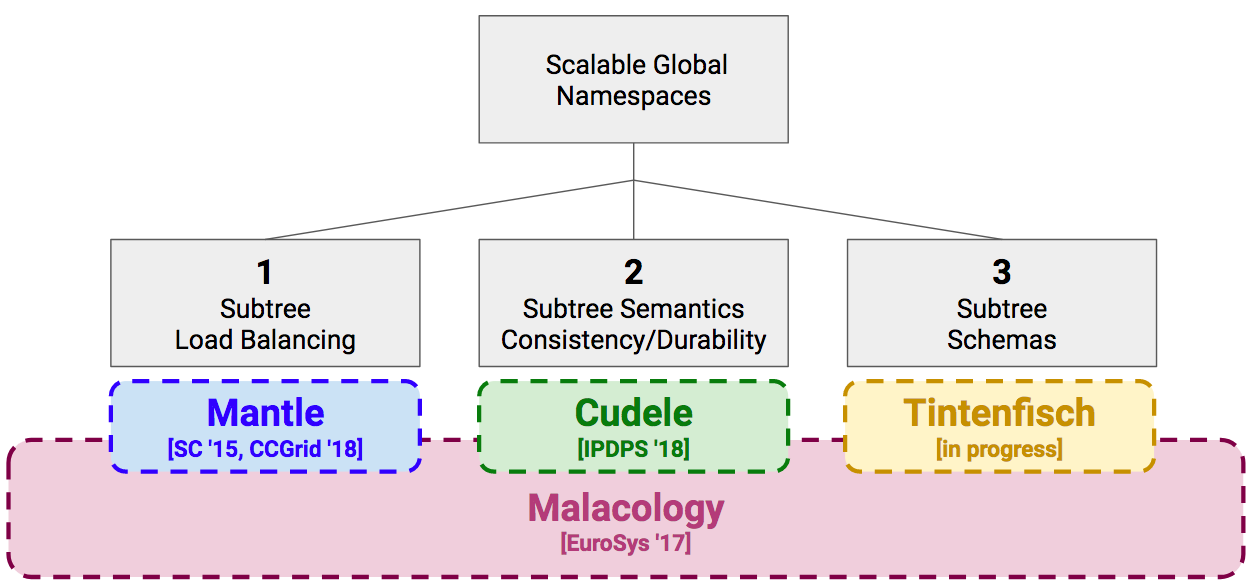
\includegraphics{figures/overview.png}
\caption{Scalable storage systems have storage daemons which store data,
monitor daemons (M) that maintain cluster state, and service-specific daemons
(e.g., file system metadata servers). Malacology enables the programmability of
internal abstractions (bold arrows) to re-use and compose existing subsystems.
With Malacology, we built new higher-level services, ZLog and Mantle, that sit
alongside traditional user-facing APIs (file, block,
object).}\label{fig:overview}
\end{figure}

A{\let\thefootnote\relax\footnote{$^{\dag}$ These authors contributed equally to
this work.}} storage system implements abstractions designed to persistently
store data and must exhibit a high level of correctness to prevent data loss.
Storage systems have evolved around storage devices that often were orders of
magnitude slower than CPU and memory, and therefore could dominate overall
performance if not used carefully. Over the last few decades members of the
storage systems community have developed clever strategies to meet correctness
requirements while somewhat hiding the latency of traditional storage
media~\cite{brewer_disks_2016}. To avoid lock-in by a particular vendor, users
of storage systems have preferred systems with highly standardized APIs and
lowest common denominator abstract data types such as blocks of bytes and byte
stream files~\cite{armbrust_view_2010}.

A number of recent developments have disrupted traditional storage systems.
First, the falling prices of flash storage and the availability of new types of
non-volatile memory that are orders of magnitude faster than traditional
spinning media are moving overall performance bottlenecks away from storage
devices to CPUs and networking, and pressure storage systems to shorten their
code paths and incorporate new
optimizations~\cite{gray_tape_2007,gray_flash_2008}.  Second, emerging ``big
data'' applications demand interface evolution to support flexible consistency
as well as flexible structured data
representations.~\cite{apache_contributors_parquet_2014}.  Finally,
production-quality scalable storage systems available as open source software
have established and are continuing to establish new, \emph{de-facto} API
standards at a faster pace than traditional standards
bodies~\cite{snia_implementing_2014,linux_foundation_kinetic_2015}.

The evolutionary pressure placed on storage systems by these trends raises the
question of whether there are principles that storage systems designers can
follow to evolve storage systems efficiently, without jeopardizing years of
code-hardening and performance optimization efforts.  In this paper we
investigate an approach that focuses on identifying and exposing existing
storage system resources, services, and abstractions that in a generalized form
can be used to \emph{program} new services. This `dirty-slate' approach of
factoring out useful code lets programmers re-use subsystems of the back-end
storage system, thus inheriting their optimizations, established correctness,
robustness, and efficiency. `Clean-slate' approaches could be implemented
faster but they do so at the expense of ``throwing away" proven code.

{\it \textbf{Contribution 1:}} We define a programmable storage system to be a
storage system that facilitates the re-use and extension of existing storage
abstractions provided by the underlying software stack, to enable the creation
of new services via composition.  A programmable storage system can be realized
by exposing existing functionality (such as \newcommentone{file system and
cluster} metadata services and synchronization and monitoring capabilities) as
interfaces that can be ``glued together'' in a variety of ways using a
high-level language. Programmable storage differs from \emph{active
storage}~\cite{riedel:vldb98}---the injection and execution of code within a
storage system or storage device---in that the former is applicable to any
component of the storage system, while the latter focuses at the data access
level. Given this contrast, we can say that active storage is an example of how
one internal component (the storage layer) is exposed in a programmable storage
system.  \addressesissue{4}

To illustrate the benefits and challenges of this approach we have designed and
evaluated Malacology, a programmable storage system that facilitates the
construction of new services by re-purposing existing subsystem abstractions of
the storage stack.  We build Malacology in Ceph, a popular open source software
storage stack.  We choose Ceph to demonstrate the concept of programmable
storage because it offers a broad spectrum of existing services, including
distributed locking and caching services provided by \newcommentone{file
system} metadata servers, durability and object interfaces provided by the
back-end object store, and propagation of consistent cluster state provided by
the monitoring service (see Figure~\ref{fig:overview}).  Malacology is
expressive enough to provide the functionality necessary for implementing new
services.  \addressesissue{4}

Malacology includes a set of interfaces that can be used as
building blocks for constructing novel storage abstractions, including:

\begin{enumerate}

\item An interface for managing strongly-consistent time-varying
\textbf{service metadata}.

\item An interface for installing and evolving domain-specific, cluster-wide
\textbf{data I/O} functionality.

\item An interface for managing access to \textbf{shared resources} using a
variety of optimization strategies.

\item An interface for \textbf{load balancing} resources across the cluster.

\item An interface for \textbf{durability} that persists policies using the
underlying storage stack's object store.

\end{enumerate}

{\it \textbf{Contribution 2:}} We implement two distributed services using
Malacology to demonstrate the feasibility of the programmable storage approach:

\begin{enumerate}

\item A high-performance distributed shared log service called ZLog, that is an
implementation of CORFU~\cite{balakrishnan_corfu_2012}

\item An implementation of Mantle, the programmable load balancing
service~\cite{sevilla:sc15-mantle}

\end{enumerate}

The remainder of this paper is structured as follows. First, we describe and
motivate the need for programmable storage by describing current practices in
the open source software community. Next we describe Malacology by presenting
the subsystems within the underlying storage system that we re-purpose, and
briefly describe how those system are used within Malacology
(Section~\ref{sec:malacology}).  Then we describe the services that we have
constructed in the Malacology framework (Section~\ref{sec:services}), and
evaluate our ideas within our prototype implementation
(Section~\ref{sec:evaluation}).  We conclude by discussing future and related
work.

\section{Application-Specific Storage Stacks}
\label{sec:application-specifc-storage-stacks}

Building storage stacks from the ground up for a specific purpose results in
the best performance. For example, GFS~\cite{ghemawat:sosp03} and
HDFS~\cite{shvachko:msst10} were designed specifically to serve MapReduce and
Hadoop jobs, and use techniques like exposing data locality and relaxing POSIX
constraints to achieve application-specific I/O optimizations. Another example
is Boxwood~\cite{maccormick:osdi04}, which experimented with B-trees and chunk
stores as storage abstractions to simplify application building.
Alternatively, general-purpose storage stacks are built with the flexibility to
serve many applications by providing standardized interfaces and tunable
parameters.  Unfortunately, managing competing forces in these systems is
difficult and users want more control from the general-purpose storage stacks
without going as far as building their storage system from the ground up.

To demonstrate a recent trend towards more application-specific storage systems
we examine the state of programmability in Ceph. Something of a storage Swiss
army knife, Ceph simultaneously supports file, block, and object interfaces on
a single cluster~\cite{ceph_contributors_ceph_2010}. Ceph's Reliable Autonomous
Distributed Object Storage (RADOS) system is a cluster of object storage
daemons that provide Ceph with data durability and integrity using replication,
erasure-coding, and scrubbing~\cite{weil_rados_2007}. Ceph already provides
some degree of programmability; the object storage daemons support
domain-specific code that can manipulate objects on the server that has the
data local.  These ``interfaces" are implemented by composing existing
low-level storage abstractions that execute atomically. They are written in C++
and are statically loaded into the system.

The Ceph community provides empirical evidence that developers are already
beginning to embrace programmable storage. Figure~\ref{fig:obj-int-dev-growth}
shows a dramatic growth in the production use of domain-specific interfaces in
the Ceph community since 2010. In that figure, classes are functional groupings
of methods on storage objects (e.g. remotely computing and caching the checksum
of an object extent).  What is most remarkable is that this trend contradicts
the notion that API changes are a burden for users.  Rather it appears that
gaps in existing interfaces are being addressed through ad-hoc approaches to
programmability. In fact, Table~\ref{table:objclasses} categorizes existing
interfaces and we clearly see a trend towards reusable services.

\begin{figure}[ht]
\centering
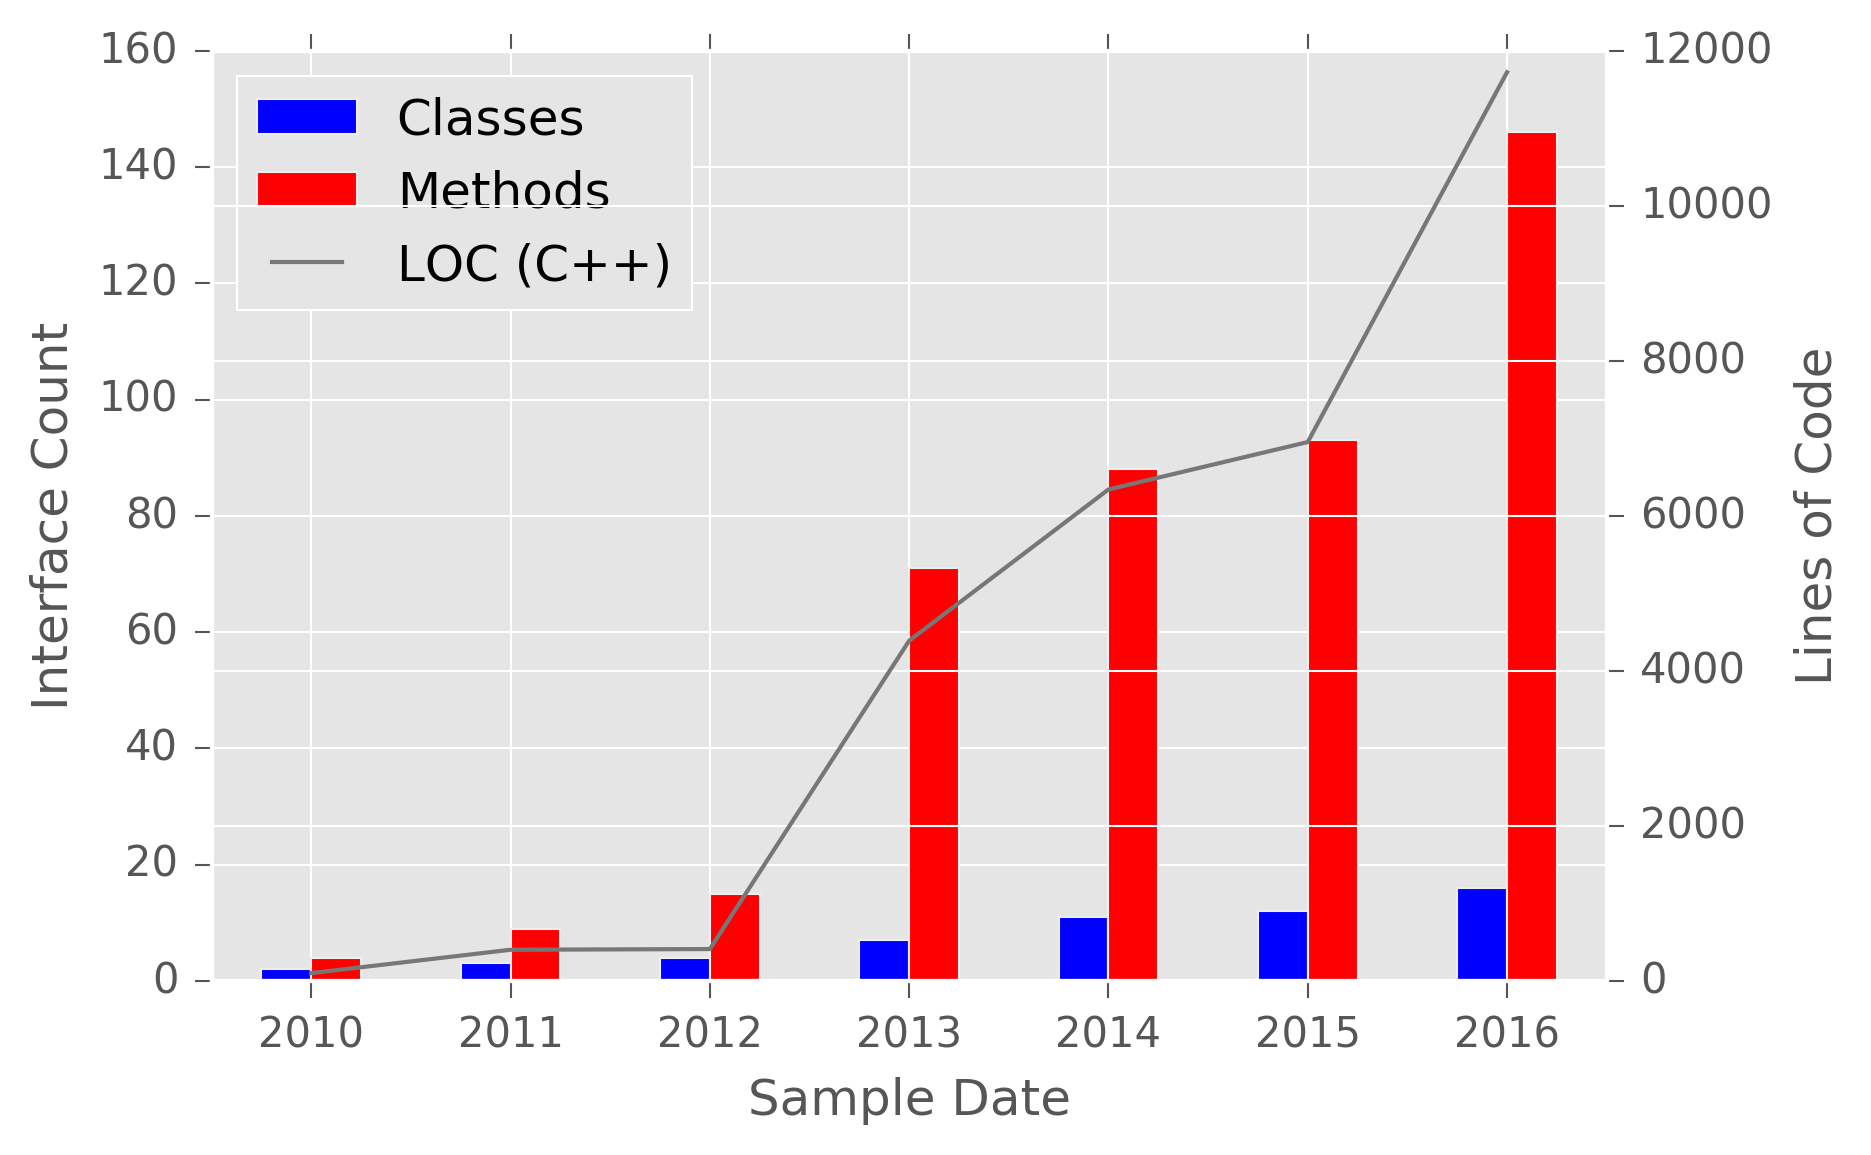
\includegraphics{figures/obj-int-dev-growth.png}
\caption{
[\href{https://github.com/michaelsevilla/malacology-popper/blob/v2.1/experiments/objclass-dev/visualize.ipynb}{source}]
Since 2010, the growth in the number of co-designed object storage interfaces
in Ceph has been accelerating. This plot is the number of object classes (a
group of interfaces), and the total number of methods (the actual API
end-points).} \label{fig:obj-int-dev-growth}
\end{figure}

\begin{table}[ht]
\centering
  \begin{tabular}{l|l|l}
    Category & Example & \# \\ \hline
    Logging  & Geographically distribute replicas & 11 \\ \hdashline
    Metadata & Snapshots in the block device OR  & \multirow{2}{*}{74} \\
    Management & Scan extents for file system repair & \\ \hdashline
    Locking  & Grants clients exclusive access & 6 \\ \hdashline
    Other & Garbage collection, reference counting  & 4\\
\end{tabular}
\caption{A variety of object storage classes exist to expose interfaces
    to applications. \# is the number of methods that implement these categories.
}
\label{table:objclasses}
\end{table}

The takeaway from Figure~\ref{fig:obj-int-dev-growth} is that programmers are
already trying to use programmability because their needs, whether they be
related to performance, availability, consistency, convenience, etc., are not
satisfied by the existing default set of interfaces. The popularity of the
custom object interface facility of Ceph could be due to a number of reasons,
such as the default algorithms/tunables of the storage system being
insufficient for the application's performance goals, programmers wanting to
exploit application-specific semantics, and/or programmers knowing how to
manage resources to improve performance. A solution based on
application-specific object interfaces is a way to work around the
traditionally rigid storage APIs because custom object interfaces give
programmers the ability to tell the storage system about their application: if
the application is CPU or I/O bound, if it has locality, if its size has the
potential to overload a single node, etc.  Programmers often know what the
problem is and how to solve it, but until the ability to modify object
interfaces, they had no way to express to the storage system how to handle
their data.

Our approach is to expose more of the commonly used, code-hardened subsystems
of the underlying storage system as interfaces. The intent is that these
interfaces, which can be as simple as a redirection to the persistent data
store or as complicated as a strongly consistent directory service, should be
used and re-used in many contexts to implement a wide range of services. By
making programmability a `feature', rather than a `hack' or `workaround', we
help standardize a development process that now is largely ad-hoc.

\section{Challenges}
\label{sec:challenges}

Implementing the infrastructure for programmability into existing services and
abstractions of distributed storage systems is challenging, even if one assumes
that the source code of the storage system and the necessary expertise for
understanding it is available.  Some challenges include:

\begin{itemize}

\item Storage systems are generally required to be highly available so that any
complete restarts of the storage system to reprogram them is usually
unacceptable.

\item Policies and optimizations are usually hard-wired into the services and
one has to be careful when factoring them to avoid introducing additional bugs.
These policies and optimizations are usually cross-cutting solutions to
concerns or trade-offs that cannot be fully explored at the time the code is
written (as they relate to workload or hardware). Given these policies and
optimizations, decomposition of otherwise orthogonal internal abstractions can
be difficult or dangerous.

\item Mechanisms that are often only exercised according to hard-wired policies
and not in their full generality have hidden bugs that are revealed as soon as
those mechanisms are governed by different policies. In our experience
introducing programmability into a storage system proved to be a great
debugging tool.

\item Programmability, especially in live systems, implies changes that need to
be carefully managed by the system itself, including versioning and propagation
of those changes without affecting correctness.

\end{itemize}

To address these challenges we present Malacology,\oldcomment{. Malacology is
both a prototype for a programmable storage system and a} \newcomment{ our
prototype programmable storage system. It uses the programmable storage}
\addressesissue{2} design approach to evolve storage systems efficiently and
without jeopardizing years of code-hardening and performance optimization
efforts.  Although Malacology uses the internal abstractions of the underlying
storage system, including its subsystems, components, and implementations, we
emphasize that our system still addresses the general challenges outlined
above.

The main challenge of designing a programmable storage system is choosing the
right internal abstractions and picking the correct layers for exposing them.
\oldcomment{In this paper, we do not present an exhaustive list of possible
internal abstractions nor do we contend that the abstractions we choose provide
the best trade-offs for all applications.} \newcomment{A programmable storage
system is not defined by what abstractions are exposed, rather a programmable
storage system adheres to the design approach of exposing interfaces so
administrators can have better control of the storage system. The interfaces
presented in this paper are abstractions that we found useful for building our
prototype services ZLog and Mantle, yet they may not provide the best
trade-offs for all higher-level services.} \addressesissue{2} For example, if
consensus is correctly exposed one could implement high-level features like
versioning, serialization, or various flavors of strongly consistent data
management on top; but perhaps a low-level consensus interface is suited well
for a particular set of applications.  These questions are not answered in this
paper and instead we focus on showing the feasibility of building such a
system, given advances in the quality and robustness of today's storage stacks.

The Malacology prototype we present has been implemented on Ceph.  While there
are other systems on top of which Malacology could be implemented (see
Table~\ref{table:examples}), we choose Ceph because it is a production quality
system and because it is open source. The large developer community ensures
that code is robust and the visibility of the code lets us expose any interface
we want. In the next section we describe the Ceph components that we expose as
Malacology interfaces.

\section{Malacology: A Programmable Storage System}
\label{sec:malacology}

\begin{table*}
\centering\small
\begin{tabular}{ l | c | l | l | l }
%\multicolumn{4}{c}{\Large \textbf{Common Internal Abstractions}} \\
\multicolumn{4}{c}{} \\
\textbf{Interface}                      &
\textbf{Section}                        &
\textbf{Example in Production Systems}  &
\textbf{Example in Ceph}                &
\textbf{Provided Functionality}            \\ \hline
Service Metadata
  & \S\ref{sec:service-metadata-interface}
  & Zookeeper/Chubby coordination~\cite{hunt_zookeeper_2010,burrows_chubby_2006}
  & cluster state management~\cite{website:ceph-mon}
  & consensus/consistency
  \\
Data I/O
  & \S\ref{sec:data-io-interface}
  & Swift in situ storage/compute~\cite{website:zerocloud}
  & object interface classes~\cite{website:cls-lua}
  & transaction/atomicity
  \\
Shared Resource
  & \S\ref{sec:shared-resource-interface}
  & MPI collective I/O, burst
  & POSIX metadata protocols
  & serialization/batching
  \\
File Type
  & \S\ref{sec:file-type-interface}
  & MPI supports architecture-specific code~\cite{thakur:iopads1999}
  & file striping strategy
  & data/metadata access
  \\
Load Balancing
  & \S\ref{sec:load-balancing-interface}
  & VMWare's VM migration~\cite{vmware-drs,gulati:hotcloud2011-cloud-resource-management} 
  & migrate POSIX metadata~\cite{weil:sc2004-dyn-metadata}
  & migration/sampling
  \\
Durability
  & \S\ref{sec:durability}
  & S3/Swift interfaces (RESTful API)
  & object store library~\cite{weil_rados_2007}
  & persistence/safety
  \\
\end{tabular}
\caption{Common internal abstractions. The same ``internal abstractions" are
common across large-scale systems because they provide functionality that
solves general distributed systems problems.  Here we list examples of what
these internal abstractions are used for in ``production systems" and in Ceph.
Malacology provides these internal abstractions as interfaces
\newcomment{(Section~\ref{sec:malacology})} that higher level
\oldcomment{applications} \newcomment{services (Section~\ref{sec:services})}
can use.  \oldcomment{; {\it italicized abstractions} are interfaces discussed
in this paper.}}
\addressesissue{1}
\label{table:examples}
\end{table*}

The guiding principle is to re-use existing services and compose them so that
these services can be \emph{programmed}. We accomplish programmability of a
service by exporting bindings for an interpreted programming language so that
programming can occur without having to restart the storage system (see also
below, Section~\ref{sec:durability}). Table~\ref{table:examples} shows the
internal services from Ceph that we expose in the Malacology prototype via
Lua~\cite{ierusalimschy1996lua} bindings\oldcomment{.} \newcomment{and
Figure~\ref{fig:implementation-overview} compares what was already present in
Ceph (gray boxes) to the Malacology interfaces we added.
Section~\ref{sec:services} will describe the higher-level services we built
with these interfaces.} \addressesissue{1}

\begin{figure}[tbp]
\centering
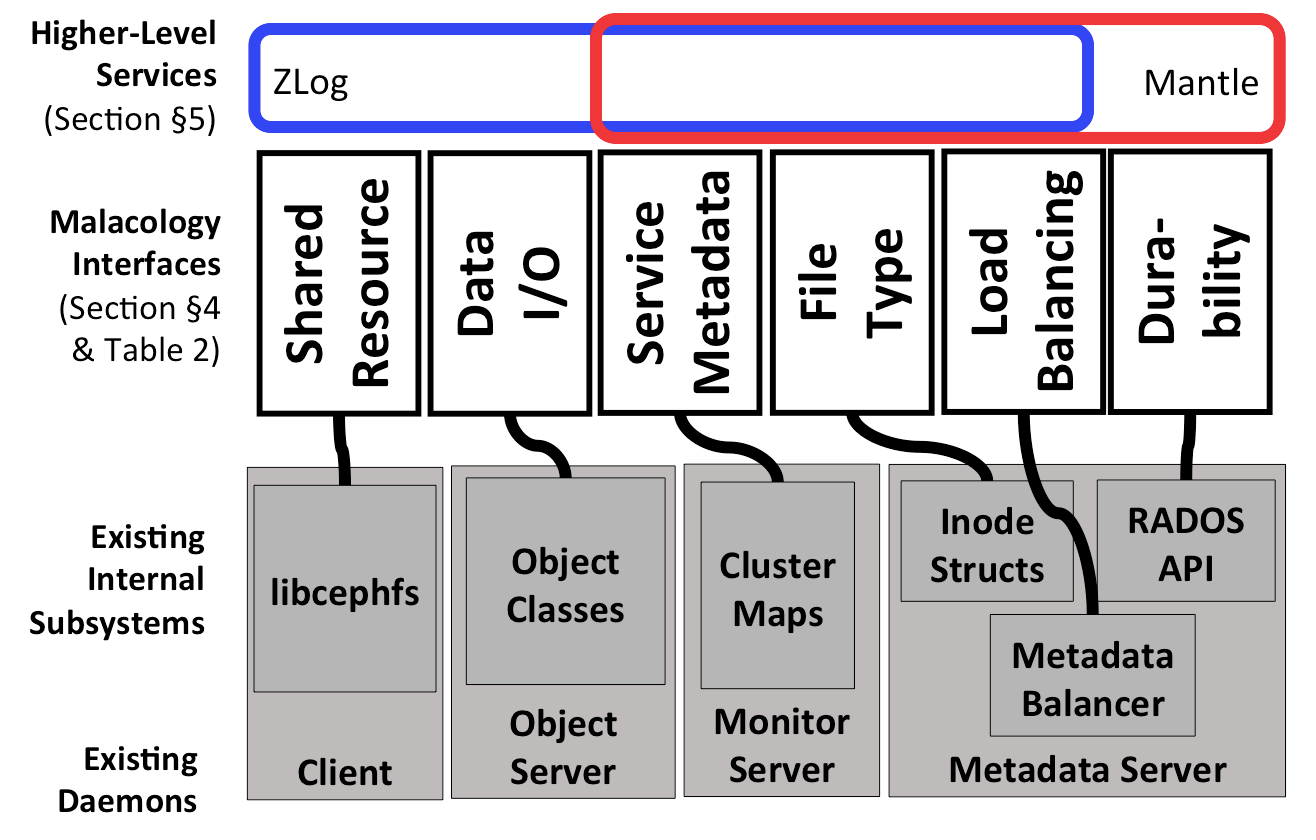
\includegraphics{figures/implementation-overview.png}
\caption{\newcomment{Malacology is implemented on the daemons and clients that
run in a Ceph cluster. Interfaces expose internal subsystems and are used as
building blocks for higher-level services.}\addressesissue{1}
\label{fig:implementation-overview}}
\end{figure}

Lua is a portable embedded scripting language and we choose it as the
interpreted language for Malacology because it offers superior performance and
productivity trade-offs, including a JIT-based implementation that is well
known for near native performance. Additionally, Lua has been used extensively
in game engines, and systems research \cite{neto:dls14-luaos}, including
storage systems where it has been effectively used both on
\cite{grawinkel:pdsw2012-lua,watkins2013:bdmc13-in-vivo,geambasu_comet_2010}
and off \cite{sevilla:sc15-mantle} the performance critical path. Finally, the
flexibility of the runtime allows execution sandboxing in order to address
security and performance concerns. We will now discuss the common subsystems
used to manage storage systems and how Malacology makes them programmable.

\subsection{Service Metadata Interface}
\label{sec:mon}
\label{sec:service-metadata-interface}
\label{service-metadata}

% straw man example
Keeping track of state in a distributed system is an essential part of any
successful service and a necessary component in order to diagnose and detect
failures, when they occur. This is further complicated by variable propagation
delays and heterogeneous hardware in dynamic environments.
\newcommentone{Service metadata is information about the daemons in the system
and includes membership details, hardware layout (e.g., racks, power supplies,
etc.), data layout, and daemon state and configuration. It differs from
traditional file system metadata which is information about files. For the rest
of the paper when we use the phrase ``metadata server" or ``metadata service",
we are referring to the daemon(s) that manages file system metadata (not
service metadata).} \addressesissue{4}

\newcomment{\\ \noindent\it{\textbf{Existing Ceph Implementation: }}} 
a consistent view of cluster state among server daemons and
clients is critical to provide strong consistency guarantees to clients.  Ceph
maintains cluster state information in per-subsystem  data structures called
``maps'' that record membership and status information.  A
Paxos~\cite{lamport_parttime_1998} monitoring service is responsible for
integrating state changes into cluster maps, responding to requests from
out-of-date clients and synchronizing members of the cluster whenever there is
a change in a map so that they all observe the same system state. As a
fundamental building block of many system designs, consensus abstractions such
as Paxos are a common technique for maintaining consistent data versions, and
are a useful system to expose.

The default behavior of the monitor can be seen as a Paxos-based notification
system, similar to the one introduced in~\cite{burrows_chubby_2006}, allowing
clients to identify when new values (termed epochs in Ceph) are associated to
given maps.  Since Ceph does not expose this service directly, as part of our
Malacology implementation, we expose a key-value service designed for managing
\oldcommentone{configuration} \newcommentone{service} metadata that is built on
top of the consensus engine. Since the monitor is intended to be out of the
high-performance I/O path, a general guideline is to make use of this
functionality infrequently and to assign small values to maps.\\

\noindent{\it{\textbf{Malacology: }}} we expose a strongly-consistent view of
time-varying service metadata as an interface rather than a hidden internal
component. This is shown in Figure~\ref{fig:implementation}, where object
interfaces and load balancer policies use the Service Metadata interface.
Malacology provides a generic API for adding arbitrary values to existing
subsystem cluster maps. As a consequence of this, applications can define
simple but useful service-specific logic to the strongly-consistent interface,
such as authorization control (just specific clients can write new values) or
triggering actions based on specific values (e.g. sanitize values).  The
higher-level services we implement in Section~\ref{sec:services} make use of
this functionality to register, version and propagate dynamic code (Lua
scripts) for new object interfaces defined in storage daemons
(Section~\ref{object-data-interface}) and policies in the load balancer
(Section~\ref{malacology:mds}).  Using this service guarantees that interface
definitions are not only made durable, but are transparently and consistently
propagated throughout the cluster so that clients are properly synchronized
with the latest interfaces.\\

\noindent\newcomment{{\it{\textbf{Impact: }}} provides core functionality
because it lets daemons come to a consensus on system critical state. Bugs in
the internal subsystems or omitting this from services that need this type of
consistency affects correctness.} \addressesissue{3, 5}

%And finally, it is important to not underestimate the importance of the
%preservation of the modifications that enable a new system service. In many
%(if not all) cases, interfaces defining access to data are just as important
%as the data itself by virtue of inherently providing structural context. Thus,
%all components of a system service must be kept to the same standards of
%protection as data in the system itself.

\oldcomment{\noindent 4.2 Object I/O Interface}
\subsection{Data I/O Interface}
\label{sec:data-io-interface}
\label{object-data-interface}

Briefly described in Section~\ref{sec:application-specifc-storage-stacks}, Ceph
supports application-specific object interfaces~\cite{weil_rados_2007}. The
ability to offload computation can reduce data movement, and transactional
interfaces can significantly simplify construction of complex storage
interfaces that require uncoordinated parallel access.

\newcomment{\\ \noindent\it{\textbf{Existing Ceph Implementation: }}} an object
interface is a plugin structured similarly to that of an RPC in which a
developer creates a named function within the cluster that clients may invoke.
In the case of Ceph each function is implicitly run within the context of an
object specified when the function is called. Developers of object interfaces
express behavior by creating a composition of native interfaces or other custom
object interfaces, and handle serialization of function input and output.  A
wide range of native interfaces are available to developers such as reading and
writing to a byte stream, controlling object snapshots and clones, and
accessing a sorted key-value database. These native interfaces may be
transactionally composed along with application specific logic to create
semantically rich interfaces. An example would be an interface that atomically
updates a matrix stored in the bytestream and an index of the matrix stored in
the key-value database.\\

\begin{figure}[tbp]
\centering
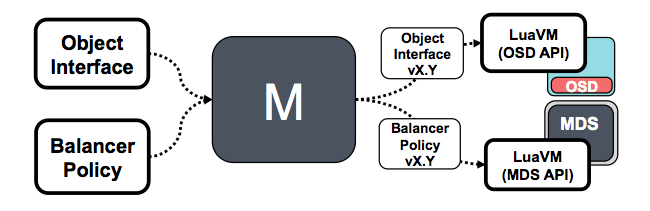
\includegraphics{figures/implementation.png}
\caption{Malacology allows users to dynamically define
object/\newcommentone{file system} metadata interfaces by composing the object
storage daemon (OSD) and metadata server (MDS) subsystems with an embedded Lua
VM.  It uses the Service Metadata interface in the monitor (M) to propagate
interfaces/versions across the cluster \label{fig:implementation}}
\end{figure}

\noindent {\it{\textbf{Malacology: }}} the implementation of Ceph's object
abstraction, although powerful, does not readily support programmability.
Supporting only C/C++ for object interface developers, Ceph requires
distribution of compiled binaries for the correct architecture, adding a large
barrier of entry for developers and system administrators. Second, having no
way to dynamically unload modules, any changes require a full restart of a
storage daemon which may have serious performance impacts due to loss of cached
data. And finally, the security limitations of the framework limit the use of
object interfaces to all but those with administrative level access and deep
technical expertise.

To address these concerns, Malacology takes advantage of Lua extensions
contributed by the Ceph community. This allows new object interfaces to be
dynamically loaded into the system and modified at runtime, resulting in a
object storage API with economy of expression, which at the same time provides
the full set of features of the original object interface implementation. New
object interfaces that are expressed in thousands of lines of code can be
implemented in approximately an order of magnitude less
code~\cite{geambasu_comet_2010}. While the use of Lua does not prevent
deployment of malicious code, certain types of coding mistakes can be handled
gracefully, and access policies are used to limit access to trusted
users~\cite{ierusalimschy1996lua}.

\oldcomment{All of these modifications work in tandem to implement the desired
behavior, and are typically co-designed together such that each depends on the
other to behave as expected.} \newcomment{\\ \noindent {\it{\textbf{Impact: }}}
helps applications optimize performance by pushing behavior to lower parts of
the storage stack, thereby minimizing hops and distributing computation.}
\addressesissue{3, 5}

\subsection{Distributed Metadata Interfaces}
\begin{notes}
\textcolor{red}{This section has been re-organized}
\end{notes}
\label{sec:distributed-metadata-interfaces}
\label{malacology:mds}

\oldcomment{The distributed metadata service in Ceph provides clients with a
POSIX file system abstraction~\cite{weil:sc2004-dyn-metadata}.}
\newcomment{File systems provide clients with the familiar POSIX file
abstraction.  While this guarantees strong consistency it comes at the cost of
scalability, increased complexity, and lower performance.} \addressesissue{1}
In general, distributed file systems protect resources by providing
hierarchical indexing and distributed locking services.  

%The metadata cluster moves units of the namespace called directory fragments
%and assigns them to servers using its own metadata load balancer. It then uses
%a hard-coded policy to balance these fragments using a scalarized load metric
%based on CPU, workload, and file system operation metrics. Although the CephFS
%balancer has been shown to be complicated, its complexity is justifiable.
%Having the flexibility to choose what to move, where to move it, and how much
%to move is very powerful. The problem is that it is difficult to pick a
%one-size-fits-all policy, system administrators may want to partition load
%based on SLAs, or applications are better equipped to make these decisions,
%etc. -- but we choose instead to expose a balancing API at strategic points in
%the balancing logic using Lua hooks. ~\cite{sevilla:sc15-mantle}. 

\oldcomment{\it{\textbf{Malacology:}} Interfaces are added in strategic spots
in the \newcommentone{file system} metadata servers for guarding shared
resources, defining new file types, and load balancing.}

\oldcomment{\noindent Shared resource interface.}
\subsubsection{Shared Resource Interface}
\label{sec:shared-resource-interface}

File system metadata servers manage client sessions, allowing
clients to obtain locks (e.g. file byte ranges), and capabilities (e.g. to
cache file data). Clients and metadata servers use a cooperative protocol in
which clients voluntarily release resources back to the \newcommentone{file
system} metadata service in order to implement sharing policies.

\newcomment{\\ \noindent\it{\textbf{Existing Ceph Implementation: }}}
the locking service implements a capability-based system that expresses what
data and \newcommentone{file system} metadata clients are allowed to access as
well as what state they may cache and modify locally.  While designed for the
file abstraction, indexing, locking, and caching are all common services that
are useful to a broad spectrum of applications.  Distributed applications that
share centralized resources (e.g. a database or directory) face similar
challenges which are often solved using application-specific sharding.

\newcomment{\\ \noindent\it{\textbf{Malacology: }}} while the current policy
for sharing access and voluntarily releasing resources is largely best-effort,
Malacology supports generalized policies between metadata servers and clients
that can be used to implement fairness or priority.

\newcomment{\\ \noindent {\it{\textbf{Impact: }}} provides core functionality
to protect and provide exclusive access for any shared resource. May hurt
performance if the resource in question does not require strong consistency.}
\addressesissue{3}

\oldcomment{\noindent File type interface.}
\subsubsection{File Type Interface}
\label{sec:file-type-interface}

Applications that manage large amounts of \newcommentone{file system} metadata
(e.g. users or database snapshots) often require a naming service.  The
metadata service exposes a POSIX file system hierarchy where files and
directories are represented as inode data structures.

\newcomment{\\ \noindent {\it{\textbf{Existing Ceph Implementation: }}} CephFS
is the POSIX compliant file system that uses Ceph.  Inodes are quite large (1KB
for an inode, 400 bytes for a directory entry, and 700 bytes for a directory)
and contain CephFS-specific policies like how to stripe data across RADOS.}

\newcomment{\\ \noindent {\it{\textbf{Malacology: }}}} allows new inode types
to be defined such that applications can create domain-specific interfaces to
inodes that may modify locking and capability policies. We will show how this
is used in Section~\ref{sec:seq} when we discuss a distributed shared-log built
on Malacology.

\newcomment{\\ \noindent {\it{\textbf{Impact: }}} this interface is both a
feature and a performance optimization. It is a feature because it allows
developers to add support for different  storage types, such as how to read new
file formats or what consistency semantics to use for a specific subtree in the
hierarchical namespace. It is also a performance optimization because future
programmers can add optimizations for processing specific types of files into
the inode itself.} \addressesissue{3}

%%% TODO: striping strategy is stored with the inode

\oldcomment{\noindent \bf Load balancing interface.} 
\subsubsection{Load Balancing Interface}
\label{sec:load-balancing-interface}

\newcomment{Many large scale storage systems separate file system metadata and
data I/O so that the corresponding services can scale independently. Metadata
requests transfer small amounts of data and they happen relatively frequently
so many systems employ separate file system metadata clusters.}

\newcomment{\\ \noindent {\it{\textbf{Existing Ceph Implementation: }}}}
addresses the challenge of balancing \newcommentone{file system} metadata load
with a separate metadata cluster. This cluster uses load balancing policies to
migrate directory inodes around the cluster to alleviate overloaded
servers~\cite{weil:sc2004-dyn-metadata}.  The policies use metrics based on
system state (e.g.  CPU and memory utilization) and statistics collected by the
cluster (e.g. the popularity of an inode). Ceph uses dynamic subtree
partitioning to move variable sized namespace subtrees. These units can be
shipped anywhere (i.e., to any metadata server of any capacity) at any time for
any reason. The original balancer was designed with hard-coded policies and
tunables.\\

\noindent {\it{\textbf{Malacology: }}} the existing load balancing mechanisms
are exposed through an API and programmers can customize the behavior through a
domain specific language. These mechanisms include the ability to migrate,
partition, and measure load. Using the Service Metadata and Durability
interfaces, this Load Balancing interface can safely version balancer policies,
save balancer policies in the back-end object store and centralize
warnings/errors. When combined with the File Type interface, the Load Balancing
interface can express policies for handling a variety of multi-tenant
workloads.

\newcomment{\\ \noindent {\it{\textbf{Impact: }}} helps applications optimize
performance by allowing them to specify how to partition, replicate, and
distribute metadata in response to overloaded servers.} \addressesissue{3}

\subsection{Durability Interface}
\label{sec:durability}

\newcomment{Object stores protect data using techniques like erasure coding,
replication, and data scrubbing. For scalability, many of these features are
implemented using a peer-to-peer protocol that allows object storage daemons to
operate autonomously without a centralized coordinator.\\}

\noindent{\it{\textbf{Existing Ceph Implementation: }}} provides storage by
striping and replicating data across RADOS~\cite{weil_rados_2007}, the reliable
distributed object store. RADOS protects data using common techniques such as
erasure coding, replication, and scrubbing. For example, when the number of
placement groups change, the object storage daemons re-balance and re-shard
data in the background in a process called placement group splitting. During
placement group splitting, object storage daemons communicate directly with
each other to converge on a new data layout.  In order to reduce load on the
monitoring service, the object storage daemons use a gossip protocol to
efficiently propagate changes to cluster maps throughout the system, and
autonomously initiate recovery mechanisms when failures are discovered.\\

\noindent {\it{\textbf{Malacology: }}} metadata service policies and object
storage interfaces are stored durability within RADOS and are managed by storing
references in the object server daemon maps. Since the cluster already propagates a
consistent view of these data structures, we use this service to automatically
install interfaces in object storage daemons, and install policies within the metadata server
daemons such that clients and daemons are synchronized on
correct implementations without restarting.

\newcomment{\\ \noindent {\it{\textbf{Impact: }}} this is a feature because it
adds data safety and persistence to system metadata; while nice to have it does
not necessarily effect correctness.} \addressesissue{3}



\section{Evaluation}
\label{sec:evaluation} 

%We wanted to implement CORFU and we had two choices: build it from the ground
%up or do it on top of Malacology. To show the feasability of building on
%Malacology our evaluation focuses on the 

Our evaluation demonstrates the feasibility of building new service
abstractions atop programmable storage, focusing on the performance of the
internal abstractions exposed by Malacology and used to construct the Mantle
and ZLog services. We also discuss latent capabilities we discovered in this
process that let us navigate different trade-offs within the services
themselves. First, we benchmark scenarios with high sequencer contention by
examining the interfaces used to map ZLog onto Malacology; specifically, we
describe the sequencer implementation and the propagation of object and data
interfaces interfaces.  Next, we benchmark scenarios in which the storage
system manages multiple logs by using Mantle to balance sequencers across a
cluster.

% should save this for future work, otherwise it undercuts the eval.
%Detailed system-wide performance measurements and analysis is forthcoming for
%both Mantle and ZLog, as we try to find the best metadata balancing policies
%and physical design implementation trade-offs.  

Since this work focuses on the programmability of Malacology, the goal of this
section is to show that the components and subsystems that support the
Malacology interfaces provide reasonable relative performance, as well as to
give examples of the flexibility that Malacology provides to programmers.  
This section uses a principled approach for evaluating tunables of the
interfaces and the trade-offs we discuss should be acknowledged when building
higher-level services.

%As we search for the best metadata balancing policies and physical design
%implementation trade-offs, we plan to rel

\subsection{Load Balancing ZLog Sequencers with Mantle}
\label{sec:zlog-balancing}

In practice, a storage system implementing CORFU will support a multiplicity of
independent totally-ordered logs for each application.  For this scenario
co-locating sequencers on the same physical node is not ideal but building a
load balancer that can migrate the shared resource (e.g., the resource
that mediates access to the tail of the log) is a time-consuming, non-trivial
task.  It requires building subsystems for migrating resources, monitoring the
workloads, collecting metrics that describe the utilization on the physical
nodes, partitioning resources, maintaining cache coherence, and managing
multiple sequencers. The following experiments demonstrate the feasibility of
using the mechanisms of the Malacology Load Balancing interface to inherit
these features and to alleviate load from overloaded servers.

\begin{figure}[t!]
\centering
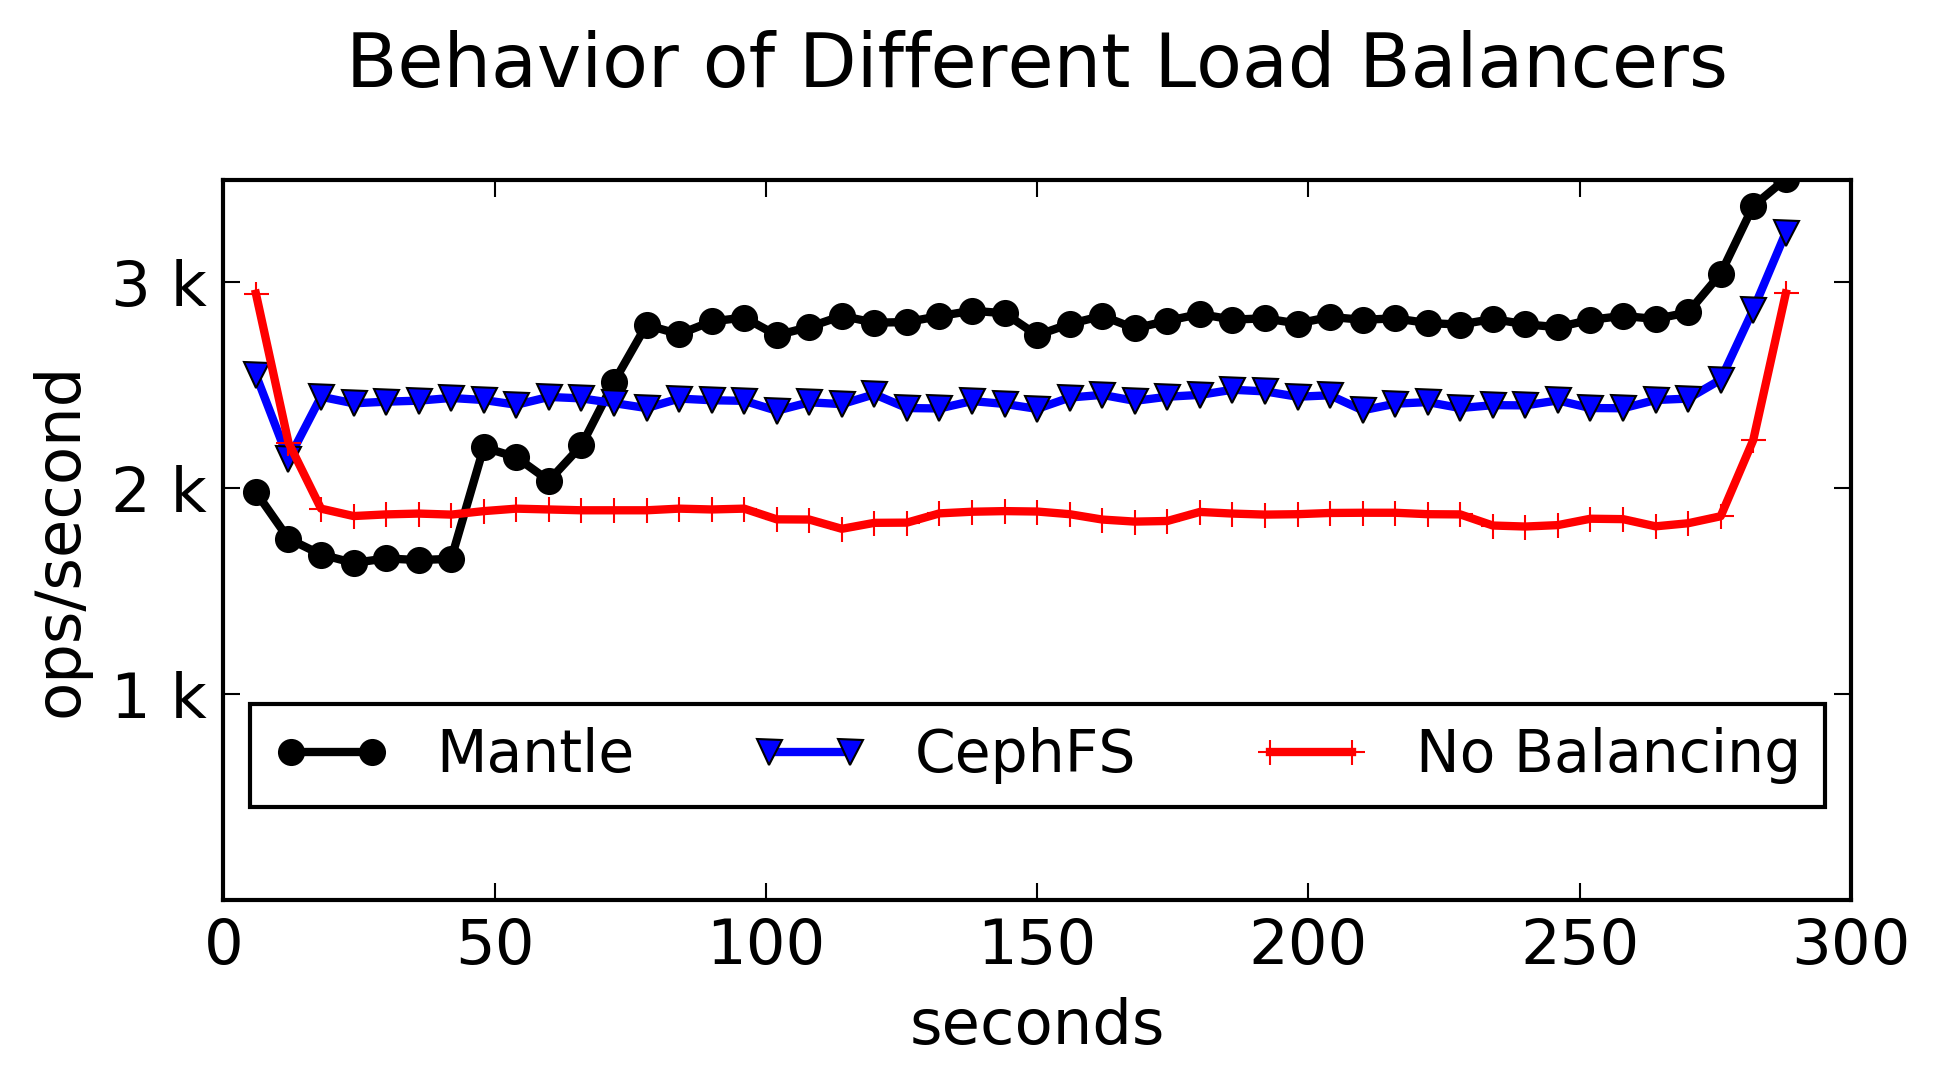
\includegraphics{./chapters/controlplane/malacology/figures/mantle-balancer-behaviors.png}
\caption{
[\href{https://github.com/michaelsevilla/malacology-popper/blob/v2.1/experiments/mds-zlog-seq-migrate-redux-3client/results-mantle-runs/visualize.ipynb}{source}]
CephFS/Mantle load balancing have better throughput than co-locating all
sequencers on the same server.  Sections~\ref{sec:feature-balancing-modes}
and~\ref{sec:feature-migration-units} quantify this improvement;
Section~\ref{sec:feature-backoff} examines the migration at 0-60 seconds.
}\label{fig:mantle-balancer-behaviors}
\end{figure}

\begin{figure}[t!]
\centering
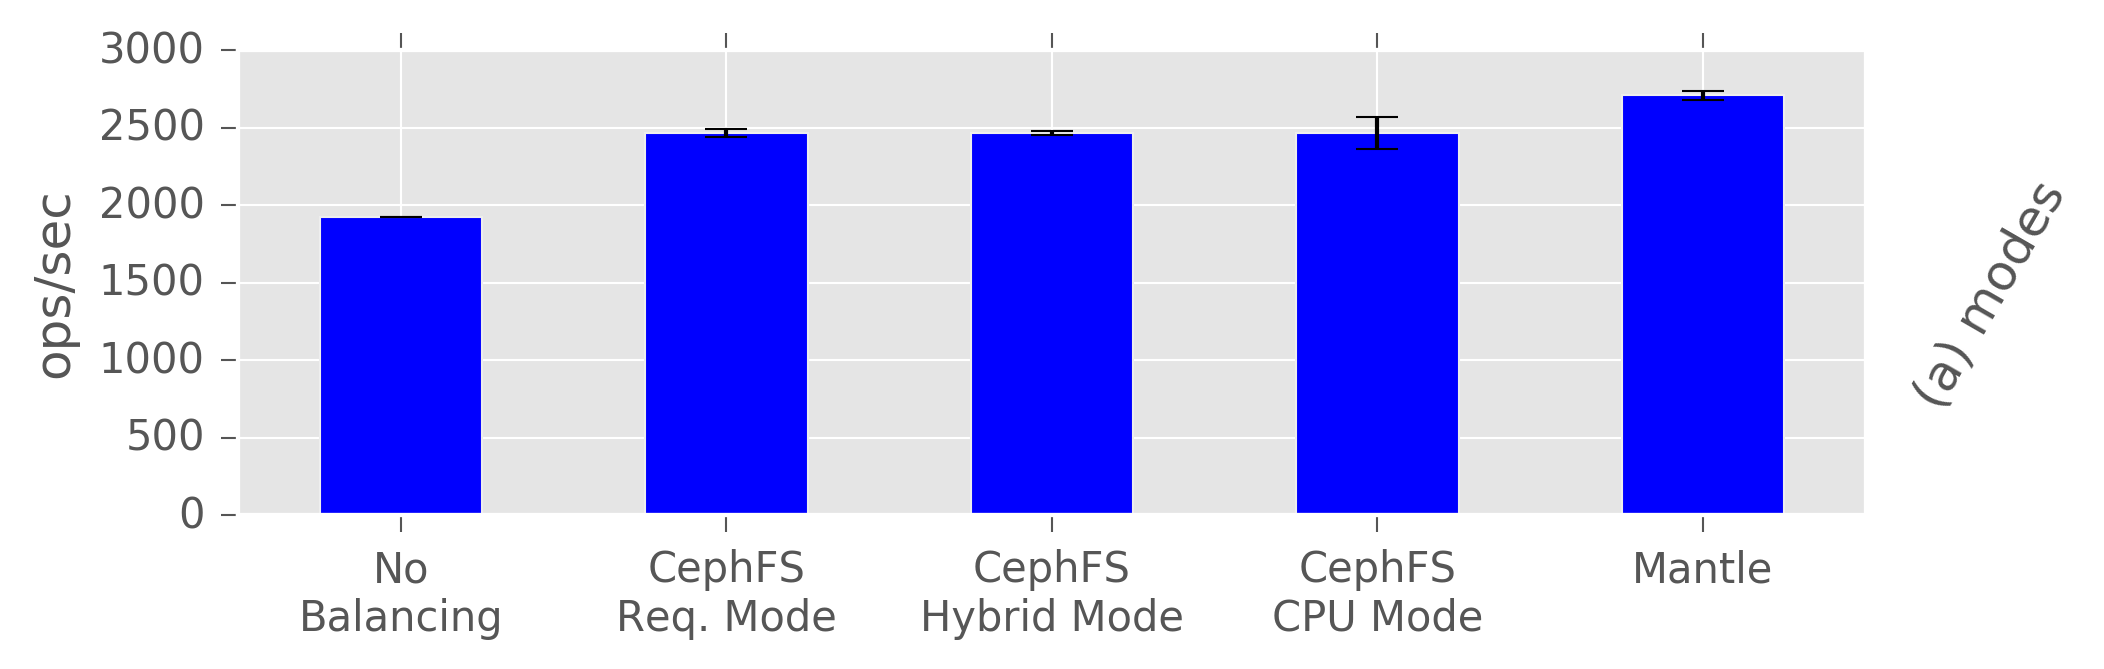
\includegraphics{./chapters/controlplane/malacology/figures/mantle-balancer-performance.png}
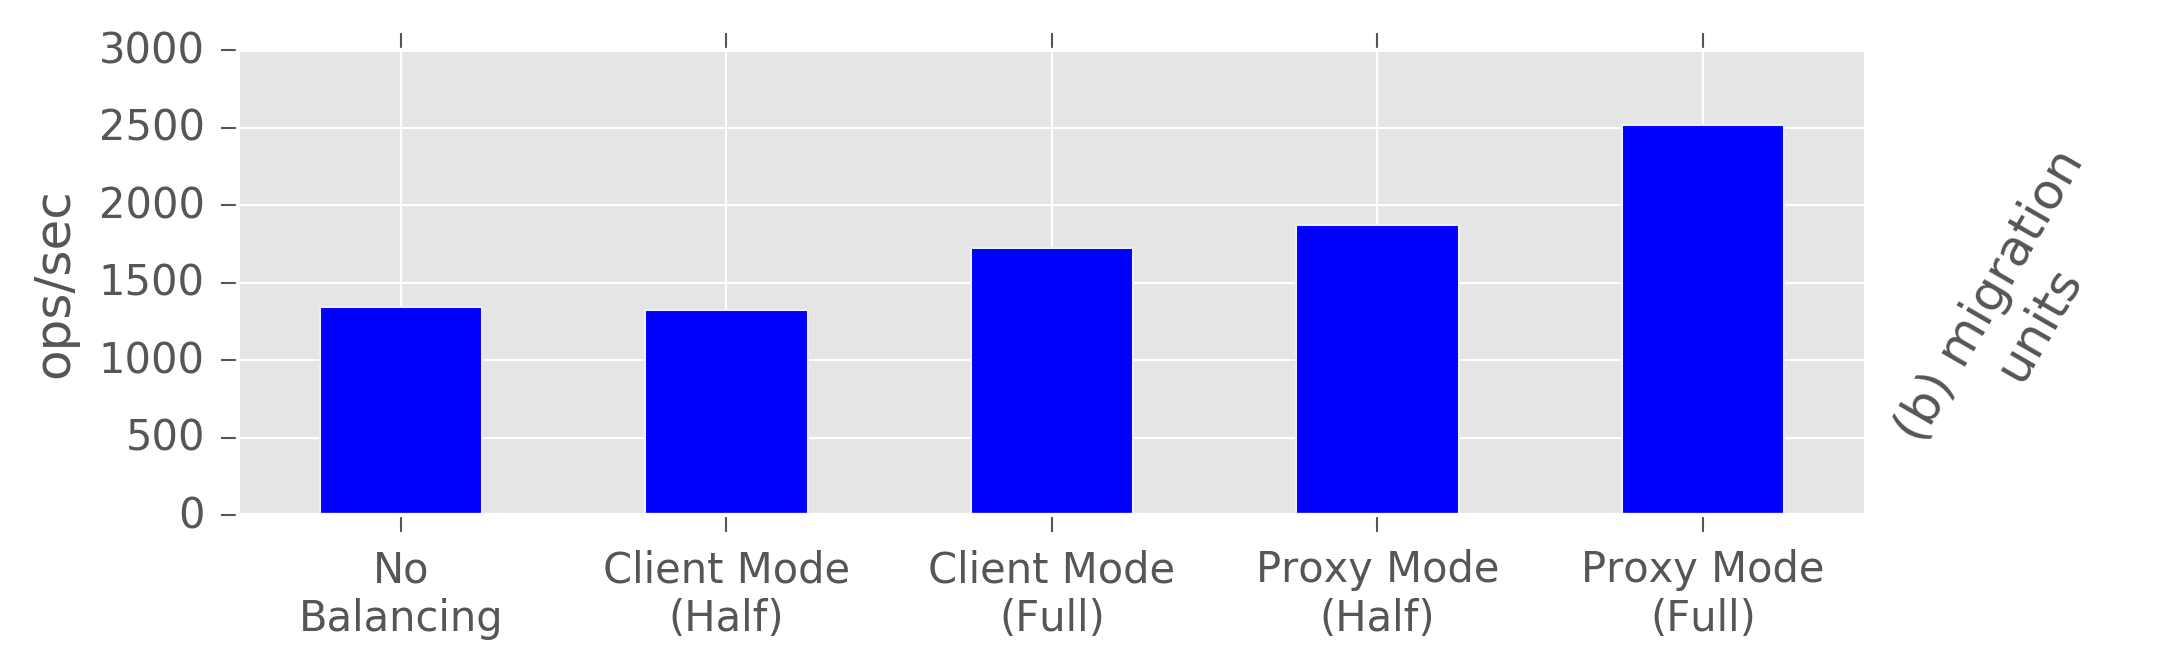
\includegraphics{./chapters/controlplane/malacology/figures/mantle-mode-performance.png}
\caption{
[\href{https://github.com/michaelsevilla/malacology-popper/blob/v2.1/experiments/mds-zlog-seq-migrate-redux-3client/results-mantle-runs/visualize.ipynb}{source},
\href{https://github.com/michaelsevilla/malacology-popper/blob/v2.1/experiments/mds-zlog-seq-migrate-redux-waves/results-paper/visualize.ipynb}{source}]
In (a) all CephFS balancing modes have the same performance; Mantle uses a
balancer designed for sequencers. In (b) the best combination of mode and
migration units can have up to a 2\(\times\)
improvement.}\label{fig:mantle-balancer-performance}
\end{figure}

The experiments are run on a cluster with 10 nodes to store objects, one node
to monitor the cluster, and 3 nodes that can accommodate sequencers.  Instead
of measuring contention at the clients like
Section~\ref{sec:sequencer-implementation}, these experiments measure
contention at the sequencers by forcing clients to make round-trips for every
request. We implement this using the Shared Resource interface that forces
round-trips.  Because the sequencer's only function is to  hand out positions
for the tail of the log, the workload is read-heavy.

First, we show how the ZLog service can orchestrate multiple sequencers using
the Malacology Load Balancing interface.
Figure~\ref{fig:mantle-balancer-behaviors} shows the throughput over time of
different load balancers as they migrate 3 sequencers (with 4 clients) around
the cluster; ``No Balancing" keeps all sequencers on one server, ``CephFS"
migrates sequencers using the hard-coded CephFS load balancers, and ``Mantle"
uses a custom load balancer we wrote specifically for sequencers.  The
increased throughput for the CephFS and Mantle curves between 0 and 60 seconds
are a result of migrating the sequencer(s) off overloaded servers.

In addition to showing that migrating sequencers improves performance,
Figure~\ref{fig:mantle-balancer-behaviors} also demonstrates features that we
will explore in the rest of this section.
Sections~\ref{sec:feature-balancing-modes}
and~\ref{sec:feature-migration-units} quantify the differences in performance
when the cluster stabilizes at time 100 seconds and
Section~\ref{sec:feature-backoff} examines the slope and start time of the
re-balancing phase between 0 and 60 seconds by comparing the aggressiveness of
the balancers.

\subsubsection{Feature: Balancing Modes}
\label{sec:feature-balancing-modes}

Next, we quantify the performance benefits shown in
Figure~\ref{fig:mantle-balancer-behaviors}.  To understand why load balancers
perform differently we need to explain the different balancing modes that the
load balancer service uses and how they stress the subsystems that receive and
forward client requests in different ways. In
Figure~\ref{fig:mantle-balancer-behaviors}, the CephFS curve shows the
performance of the balancing mode that CephFS falls into {\it most of the
time}.  CephFS currently has 3 modes for balancing load: CPU mode, workload
mode, and hybrid mode. All three have the same structure for making migration
decisions but vary based on the metric used to calculate load. For this
sequencer workload the 3 different modes all have the same performance, shown
in Figure~\ref{fig:mantle-balancer-performance} (a), because the load balancer
falls into the same mode a majority of the time.  The high variation in
performance for the CephFS CPU Mode bar reflects the uncertainty of using
something as dynamic and unpredictable as CPU utilization to make migration
decisions.  In addition to the suboptimal performance and unpredictability,
another problem is that all the CephFS balancers behave the same. This prevents
administrators from properly exploring the balancing state space.

Mantle gives the administrator more control over balancing policies; for the
Mantle bar in Figure~\ref{fig:mantle-balancer-performance} (a) we use the Load
Balancing interface to program logic for balancing read-heavy workloads,
resulting in better throughput and stability.  When we did this we also
identified two balancing modes relevant for making migration decisions for
sequencers. 

Using Mantle, the administrator can put the load balancer into ``proxy mode" or
``client mode". In proxy mode one server receives all requests and farms off
the requests to slave servers; the slave servers do the actual tail finding
operation. In client mode, clients interact directly with the server that has
their sequencer.  These modes are illustrated in Figure~\ref{fig:mantle-modes}.
``No Balancing" is when all sequencers are co-located on one physical server --
performance for that mode is shown by the ``No Balancing" curve in
Figure~\ref{fig:mantle-balancer-behaviors}. In ``Proxy Mode", clients continue
sending requests to server A even though some of the sequencers have been
migrated to another server. Server A redirects client requests for sequencer 2
to server B.  ``Proxy Mode (Half)" is shown in
Figure~\ref{fig:mantle-balancer-behaviors}; in this scenario, half of the
sequencers have migrated off the first server. Alternatively, ``Proxy Mode
(Full)", which is not pictured, is when all the sequencers migrate off the
first server.  ``Client Mode", shown on the far right of
Figure~\ref{fig:mantle-modes}, shows how clients for sequencer 2 contact server
B without a redirect from server A.

\begin{figure}[t!]
\centering
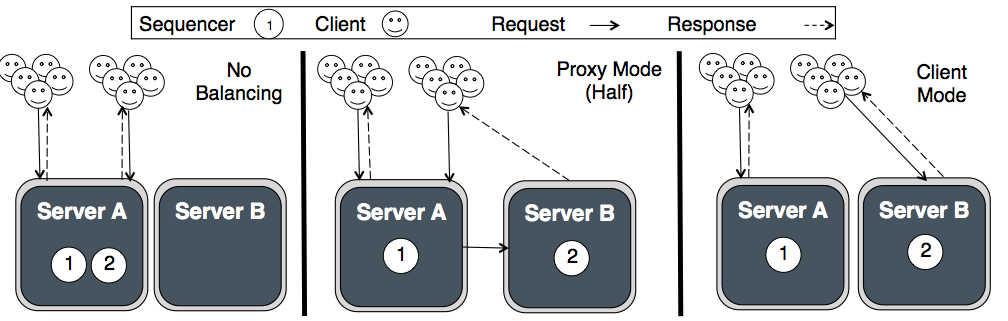
\includegraphics{./chapters/controlplane/malacology/figures/mantle-modes.png}
\caption{ In client mode clients sending requests to the server that houses
their sequencer. In proxy mode clients continue sending their requests to the
first server.  }\label{fig:mantle-modes}
\end{figure}

\begin{figure}[t!]
\centering
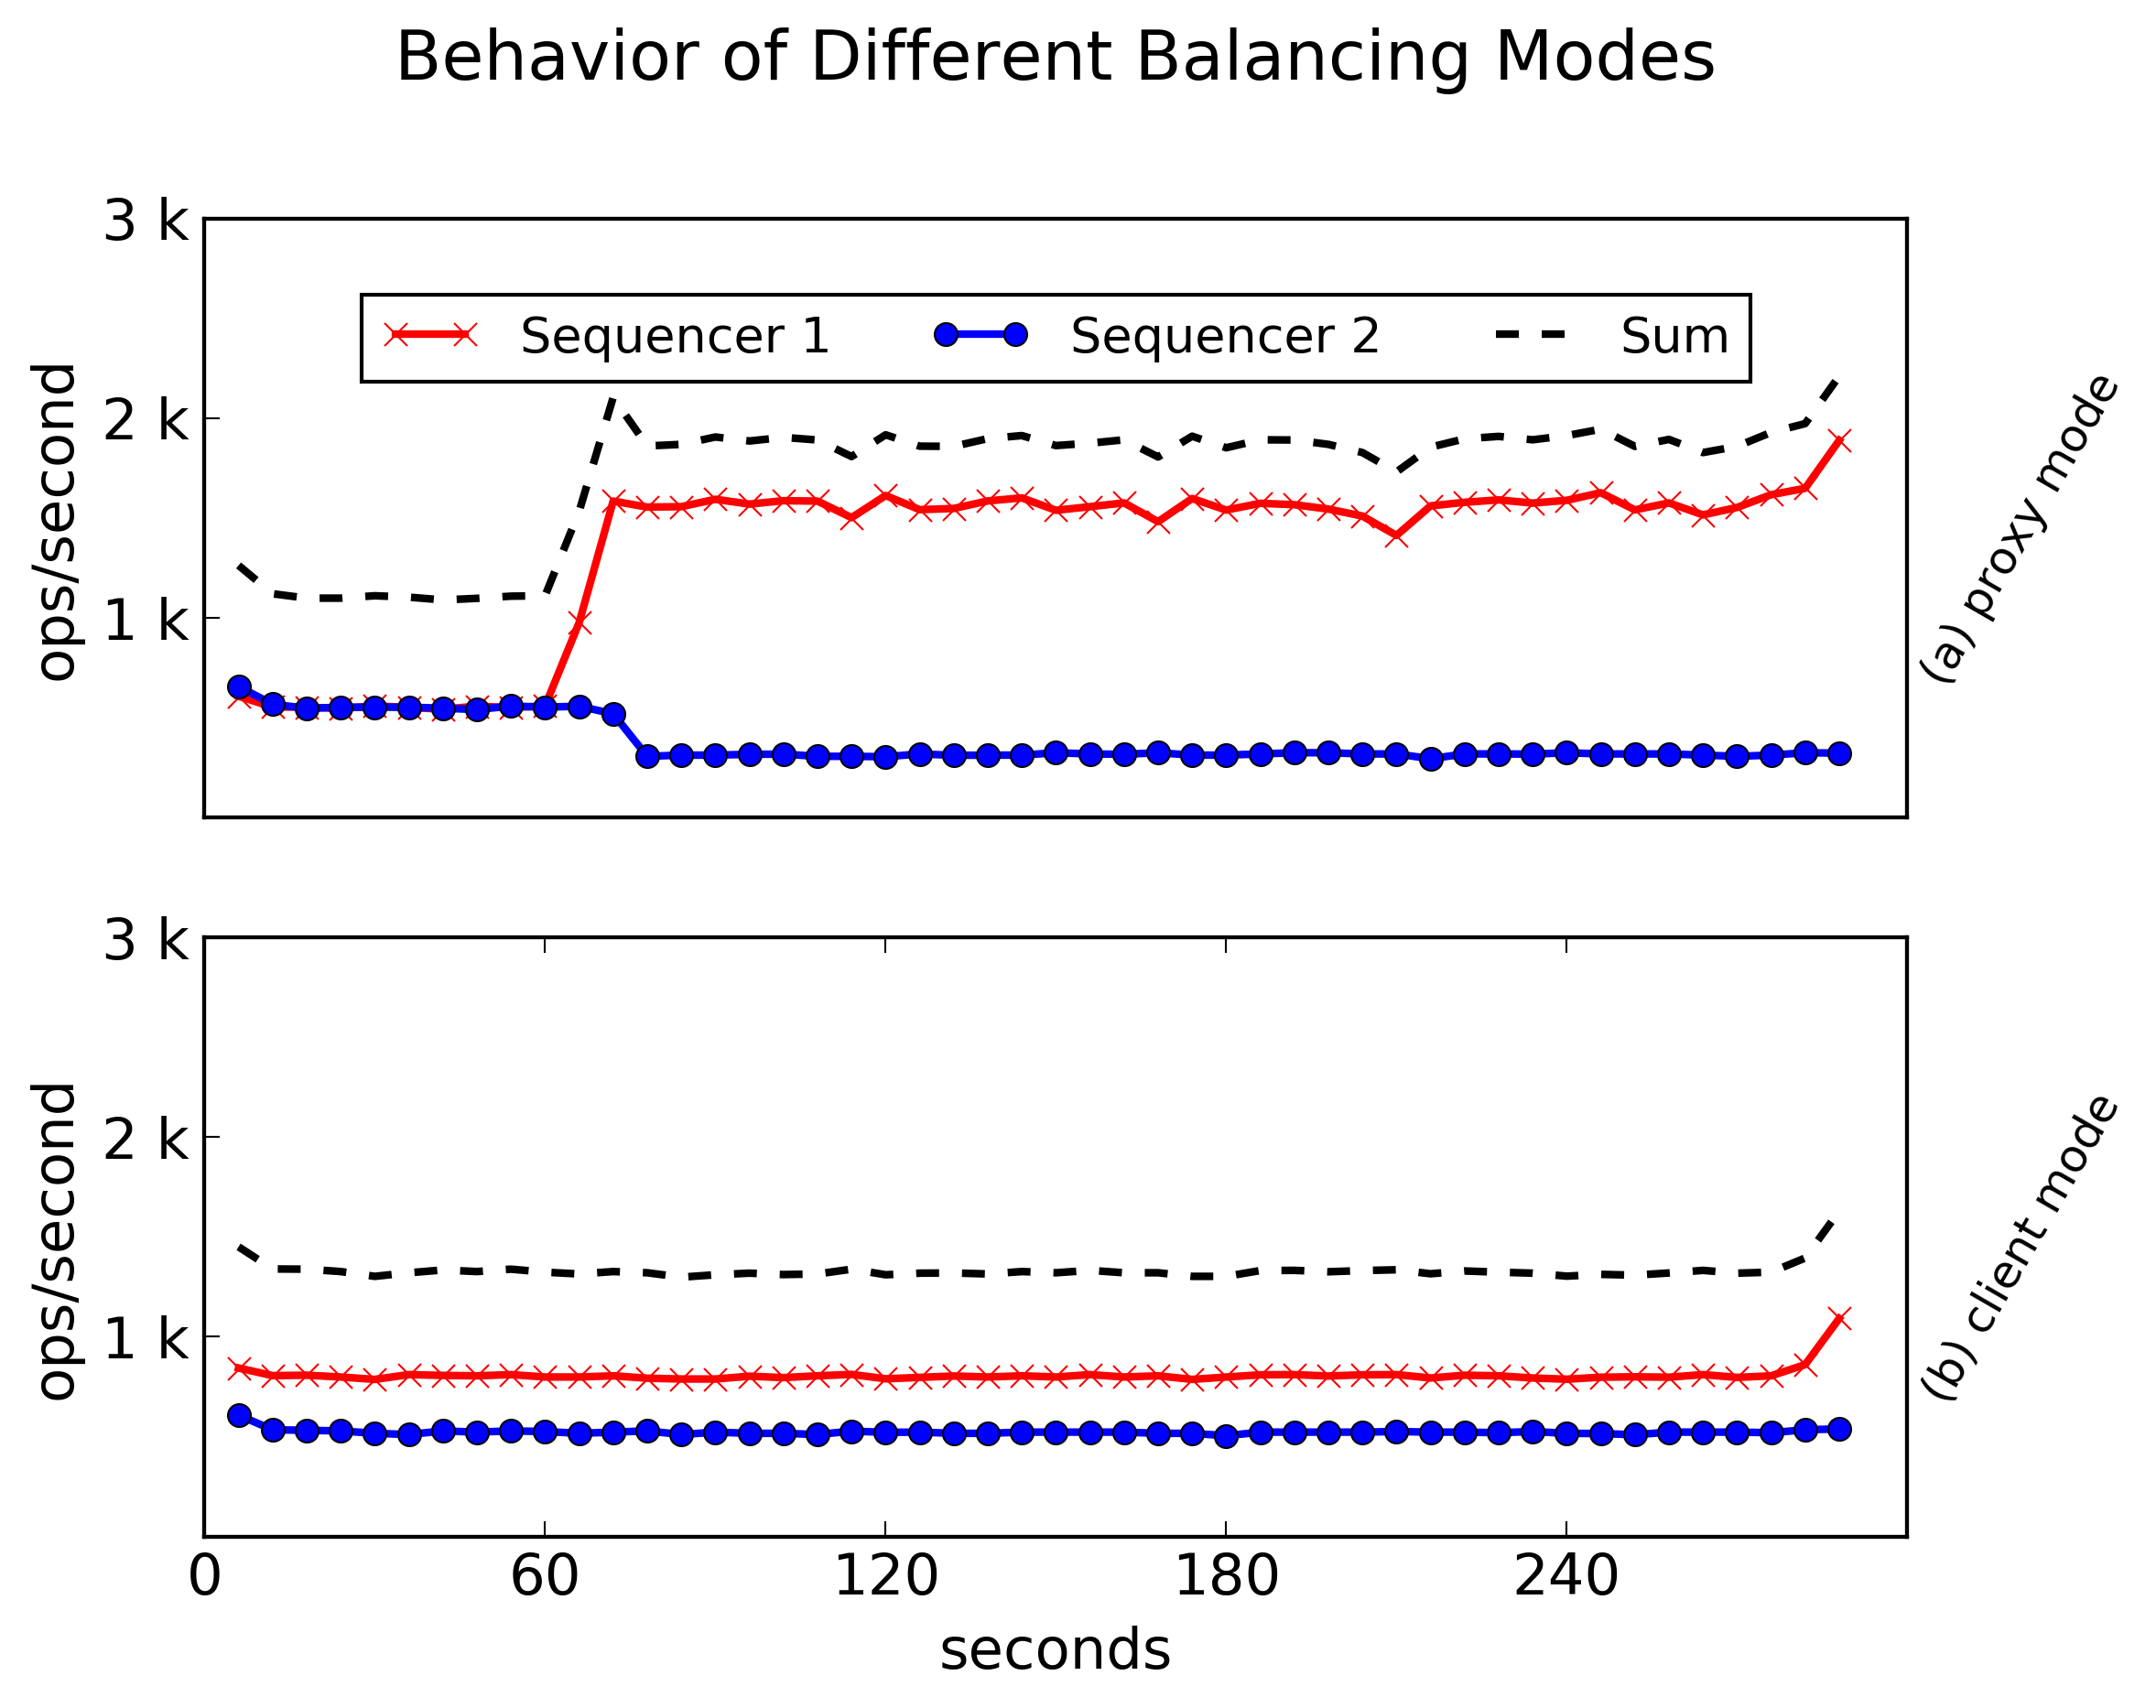
\includegraphics{./chapters/controlplane/malacology/figures/mantle-mode-behavior.png}
\caption{
[\href{https://github.com/michaelsevilla/malacology-popper/blob/v2.1/experiments/mds-zlog-seq-migrate-redux-waves/results-paper/visualize.ipynb}{source}]
The performance of proxy mode achieves the highest throughput but at the cost
of lower throughput for one of the sequencers. Client mode is more fair but
results in lower cluster throughput.  }\label{fig:mantle-mode-behavior}
\end{figure}

Figure~\ref{fig:mantle-mode-behavior} shows the throughput over time of the two
different modes for an environment with only 2 sequencers (again 4 clients
each) and 2 servers. The curves for both sequencers in
Figure~\ref{fig:mantle-mode-behavior}(a) start at less than 1000 ops/second and
at time 60 seconds Mantle migrates Sequencer 1 to the slave server.
Performance of Sequencer 2 decreases because it stayed on the proxy which now
processes requests for Sequencer 2, and forwards requests for Sequencer 1. The
performance of Sequencer 1 improves dramatically because distributing the
sequencers in this way separates (1) the handling of the client requests and
(2) finding the tail of the log and responding to clients.  Doing both steps is
too heavy weight for one server and sequencers on slave nodes can go faster if
work is split up; this phenomenon is not uncommon and has been observed in
chain replication~\cite{chain_rep}.

Cluster throughput improves at the cost of decreased throughput for Sequencer
2.  Figure~\ref{fig:mantle-mode-behavior}(b) is set to sequencer mode manually
(no balancing phase) and shows that the cluster throughput is worse than the
cluster throughput of proxy mode. That graph also shows that Sequencer 2 has
less throughput than Sequencer 1. In this case, the scatter-gather process used
for cache coherence in the metadata protocols causes strain on the server
housing Sequencer 2 resulting in this uneven performance. 

\subsubsection{Feature: Migration Units}
\label{sec:feature-migration-units}

Another factor that affects performance in this environment is how much load is
on each server; these experiments quantify that effect by programming the Load
Balancing interface to control the amount of load to migrate. We call this
metric a ``migration unit".  Expressing this heuristic is not easily achievable
with outward facing tunable parameters (i.e. system knobs) but with Mantle's
programmable interface, we can force the load balancer to change its migration
units. To force the balancer into the Proxy Mode (Half) scenario in
Figure~\ref{fig:mantle-modes}, which uses migration units equal to half the
load on the current server, we can use: \texttt{ targets[whoami+1] =
mds[whoami]["load"]/2 }.

This code snippet uses globally defined variables and tables from the Mantle
API~\cite{sevilla:sc15-mantle} to send half of the load on the current server
(whoami) to the next ranked server (whoami + 1); the \texttt{targets} array is
a globally defined table that the balancer uses to do the migrations.
Alternatively, to migrate all load a time step, we can remove the division by
2.

%\begin{figure}[t!]
%\centering
%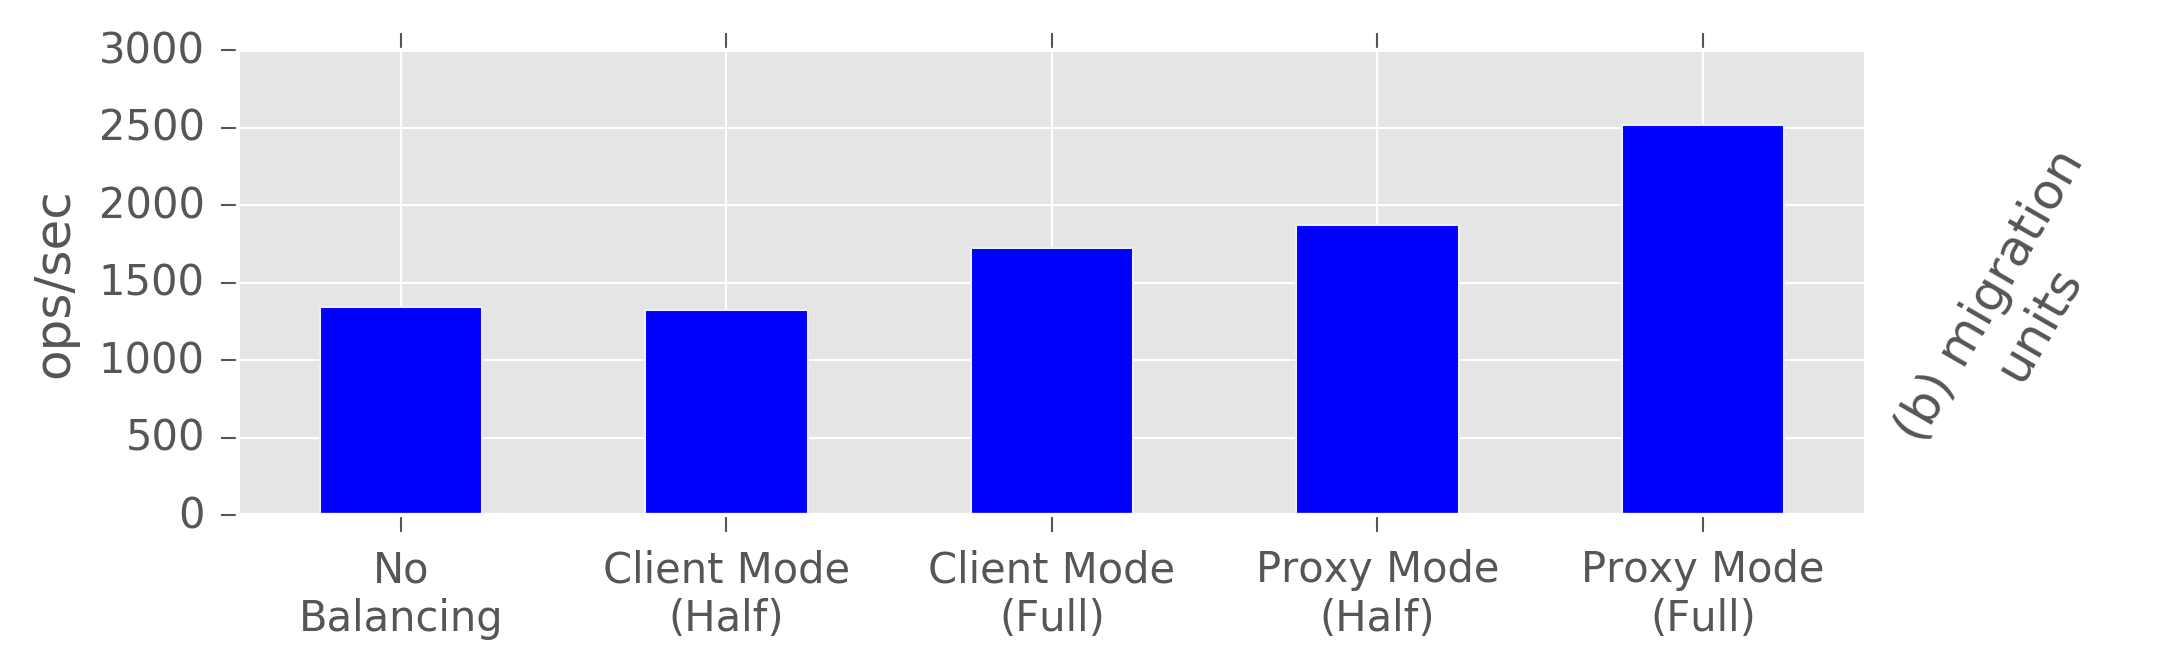
\includegraphics{./chapters/controlplane/malacology/figures/mantle-mode-performance.png}
%\caption{The performance of the different modes using various migration units
%shows almost a 2\(\times\) improvement in the best case.
%}\label{fig:mantle-mode-performance}
%\end{figure}

Figure~\ref{fig:mantle-balancer-performance} (b) shows the performance of the
modes using different migration units. Recall that this setup only has 2
sequencers and 2 servers, so performance may be different at scale. Even so, it
is clear that client mode does not perform as well for read-heavy workloads. We
even see a throughput improvement when migrating all load off the first server,
leaving the first server to do administrative tasks (this is common in the
metadata cluster because the first server does a lot of the cache coherence
work) while the second server does all the processing. Proxy mode does the
best in both cases and shows large performance gains when completely decoupling
client request handling and operation processing in Proxy Mode (Full).  The
parameter that controls the migration units helps the administrator control the
sequencer co-location or distribution across the cluster. This trade-off was
explored extensively in the Mantle paper but the experiments we present here
are indicative of an even richer set of states to explore.

\subsubsection{Feature: Backoff}
\label{sec:feature-backoff}

Tuning the aggressiveness of the load balancer decision making is also a
trade-off that administrators can control and explore. The balancing phase from
0 to 60 seconds in Figure~\ref{fig:mantle-balancer-behaviors} shows different
degrees of aggressiveness in making migration decisions; CephFS makes a
decision 10 seconds into the run and throughput jumps to 2500 ops/second 
while Mantle takes more time to stabilize. This conservative behavior is
controlled by programming the balancer to (1) use different conditions for when
to migrate and (2) using a threshold for sustained overload. 

We control the conditions for when to migrate using \texttt{when()}, a callback
in the Mantle API.  For the Mantle curve in
Figure~\ref{fig:mantle-balancer-behaviors} we program \texttt{when()} to wait
for load on the receiving server to fall below a threshold. This makes the
balancer more conservative because it takes 60 seconds for cache coherence
messages to settle.  The Mantle curve in
Figure~\ref{fig:mantle-balancer-behaviors} also takes longer to reach peak
throughput because we want the policy to wait to see how migrations affect the
system before proceeding; the balancer does a migration right before 50
seconds, realizes that there is a third underloaded server, and does another
migration. 

The other way to change aggressiveness of the decision making is to program
into the balancer a threshold for sustained overload. This forces the balancer
to wait a certain number of iterations after a migration before proceeding. In
Mantle, the policy would use the save state function to do a countdown after a
migration.  Behavior graphs and performance numbers for this backoff feature is
omitted for space considerations, but our experiments confirm that the more
conservative the approach the less overall throughput.
 
\textbf{Malacology pulls} the load balancing service out of the storage system
to balance sequencers across a cluster. This latent capability also gives
future programmers the ability to explore the different load balancing
trade-offs including: load balancing modes to control forwarding vs. client
redirection, load migration units to control sequencer distribution vs.
co-location, and backoffs to control conservative vs. aggressive decision
making.

%\subsubsection{Experiment: Object Class
%Programmability}\label{experiment-object-class-programmability}
%
%Add quote from CORFU paper that talks about what they had to hack
%
%\subsubsection{Experiment: Multi-Client
%Burstiness}\label{experiment-multi-client-burstiness}
%
%\begin{figure}[htbp] \centering
%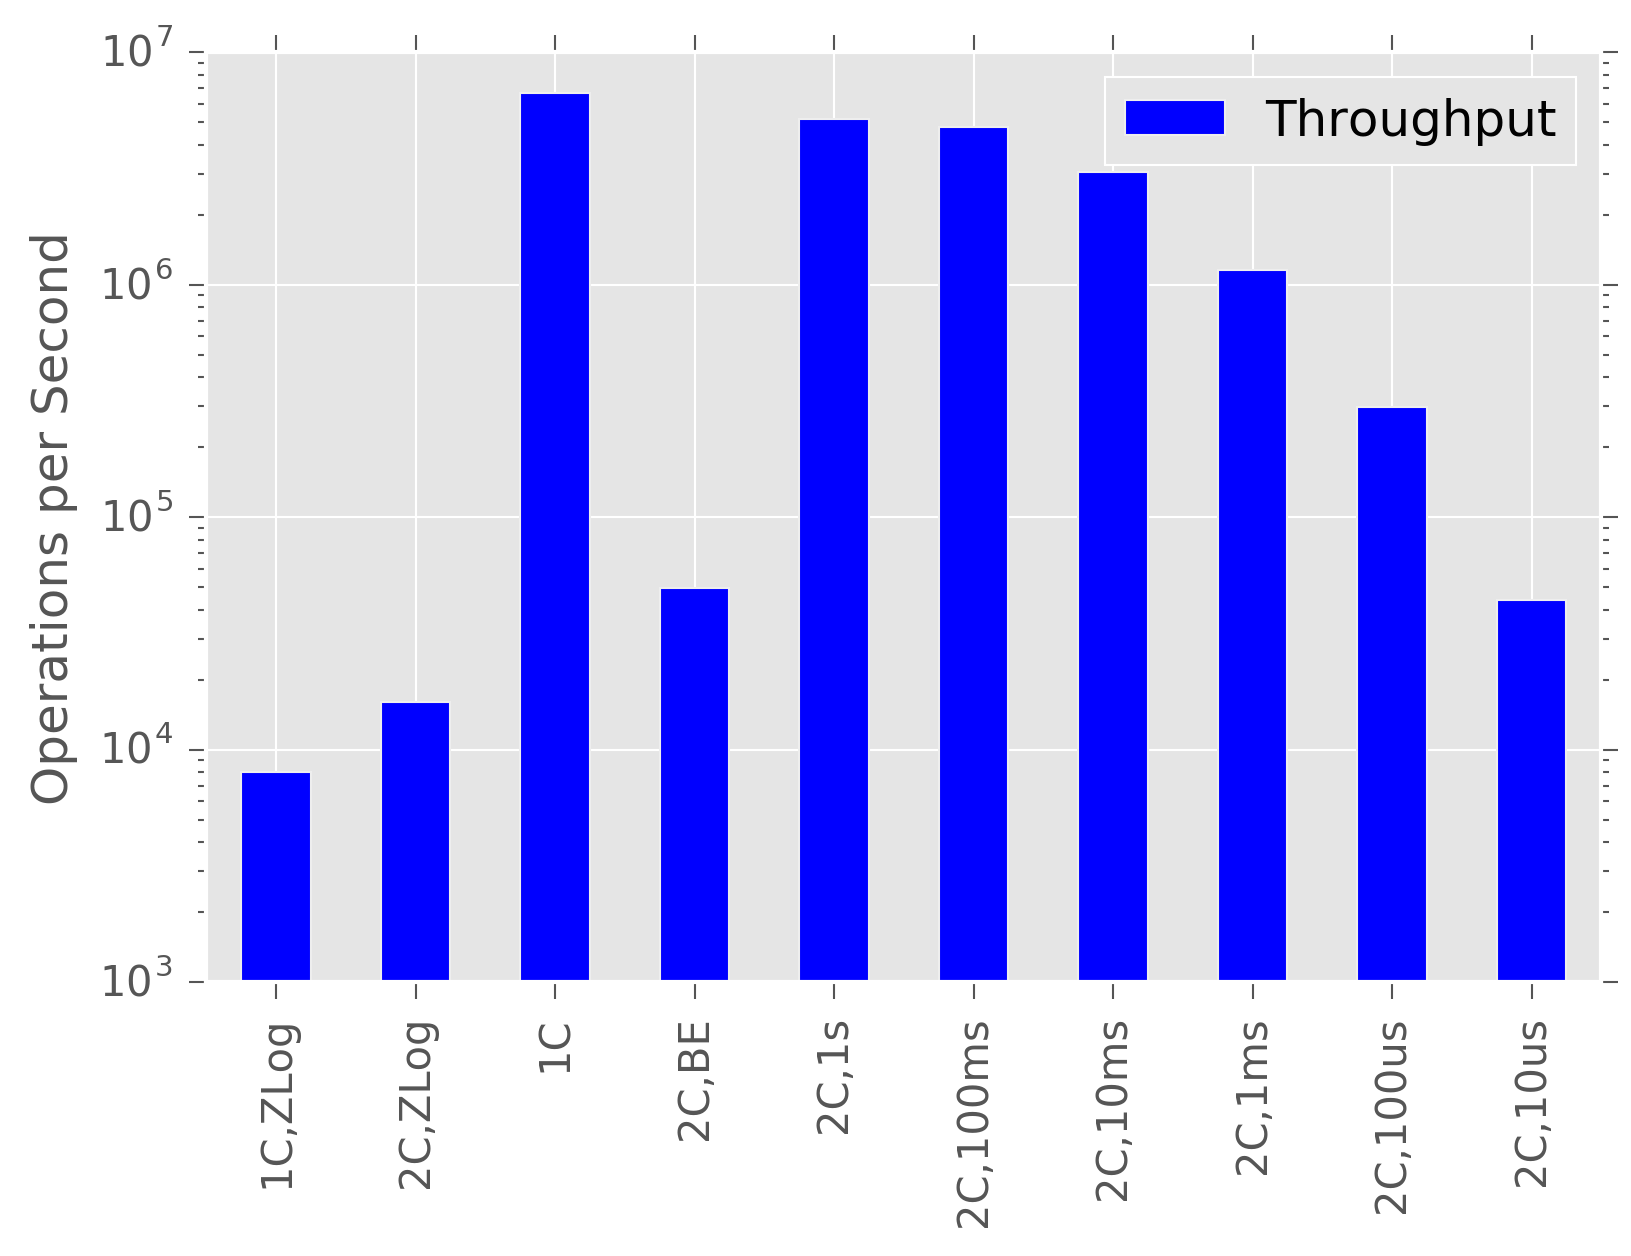
\includegraphics{./chapters/controlplane/malacology/figures/caps-delay-thruput.png} \caption{Forcing the client
%to drop their capabilities later (delay) improves throughput} \end{figure}

\section{Future Work}
 
\newcommentone{Malacology is a first step towards showing how general-purpose
storage systems can be adapted to target special-purpose applications.  By
encapsulating storage system functionality as reusable building blocks, we
enable application developers to leverage storage capabilities based on
interfaces that are proven and understandable.  However, creation and
composition of interfaces is complex; constructs must be combined safely in
order to provide correctness, performance and security. We will study
additional Malacology-based services in order to learn techniques that support
safe composition.}\addressesissue{5}
 
\newcommentone{Some higher-level services that we plan to build using the
interfaces in Table~\ref{table:examples} are: an elastic cloud database, a data
processing engine, and a data layout manager. Approaches proposed so far use
the Data I/O interface to push down predicates and computation, the File Type
interface to maintain access paths and metadata efficiently, and the Durability
interface to manage ingestion and movement. Using the programmable storage
approach helps us build higher-level services that work well with the storage
system not in spite of it.}
 
\newcommentone{ Our experience with ZLog and Mantle demonstrates that the labor
of wrapping existing services in reusable interfaces is justified by the power
and flexibility that this encapsulation affords to programmers.  In exchange
for this flexibility, however, programmers may forfeit the \emph{protection
from change} afforded by narrow storage interfaces such as the POSIX API.  To
implement applications on programmable storage systems such as Malacology,
programmers must find solutions by navigating a complex design space,
simultaneously addressing functional correctness, performance and fault
tolerance. Worse still, their solutions may be sensitive to changes in the
underlying environment, such as hardware upgrades, software version changes and
evolving workloads.  For example, a major version change in Ceph required us to
rewrite significant parts of ZLog to maintain acceptable performance. Each such
evolution costs developer time and risks introducing bugs.}
 
\newcommentone{We are actively exploring the use of high-level
\emph{declarative} languages based on Datalog~\cite{alvaro:cidr11} to program
data access and storage APIs.  Using this approach, a systems programmer can
specify the functional behavior in a relational (or algebraic) language,
allowing an optimizer to search through the space of functionally equivalent
physical implementations and select a good execution plan, re-optimizing when
storage characteristics or statistics change.  Much like query planning and
optimization in database systems~\cite{hellerstein:cidr15}, this approach will
separate the concerns of correctness and performance, protecting applications
(which usually evolve slowly) against changes in more dynamic storage system.}
\addressesissue{3}

\section{Related Work}

Programmability of operating systems and networking resources, including
distributed storage systems is not new, but we are not aware of work that makes
generalization of existing services into programmable resources a key principle
in storage systems design. 

Programmable storage systems can be viewed as an infrastructure for creating
abstractions to better separate policies from mechanisms. This idea is not new.
Software-defined networks (SDNs) create such an abstraction by separating the
control plane from the data plane (see for example~\cite{jain:sigcomm13}). This
notion of control/data separation was also applied in software-defined storage
(SDS)~\cite{thereska:sosp13,stefanovici:fast16}. Similarly,
IOStack~\cite{gracia:internet16} is providing policy-based provisioning and
filtering in OpenStack Swift. According to a SNIA white
paper~\cite{carlson:snia2014}, the primary goal of SDS is to control and
facilitate flexible and dynamic provisioning of storage resources of different
kinds, including flash memory and disk drives, to create a virtual mapping
between common storage abstractions (e.g. files, objects, and blocks) and
storage devices taking data service objectives in terms of protection,
availability, performance, and security into account. A programmable storage
system exposes internal abstractions so that end users (not necessarily
operators) can create new services on top of the storage stack. Thus, our
notion of programmable storage differs from ``software-defined storage'' (SDS)
in terms of goals and scope, although definitions of SDS are still in flux.

Another view of programmable storage systems is one of tailoring systems
resources to applications~\cite{arpaci:sosp01}. Related efforts include the
Exokernel~\cite{engler:sosp95}, SPIN~\cite{bershad:sosp95} and
Vino~\cite{seltzer:osdi96} projects; the latter two addressed the ability of
injecting code into the kernel to specialize resource management. Another
approach is to pass hints between the different layers of the I/O stack to
bridge the semantic gap between applications and
storage~\cite{arpaci:sosp01,sivathanu:fast03,mesnier:sosp11}.

Malacology uses the same Active and Typed Storage module presented in
DataMods~\cite{watkins:scc2012-datamods}; Asynchronous Service and File Manifolds
can be implemented with small changes to the Malacology framework, namely
asynchronous object calls and Lua stubs in the inode, respectively.

\section{Conclusion}
\label{conclusion-and-future-work}

Programmable storage is a viable method for eliminating duplication of complex
error-prone software used as workarounds for storage system deficiencies. We
propose that systems expose their services in a safe way allowing application
developers to customize system behavior to meet their needs while not
sacrificing correctness. To illustrate the benefits of this approach we
presented Malacology\footnote{\url{http://programmability.us}}, a programmable
storage system that facilitates the construction of new services by
re-purposing existing subsystem abstractions of the storage stack. 

\oldcommentone{Future work will focus on constructing more interfaces to
support a wide variety of storage system services that can be configured
on-the-fly in existing systems. This work is one point along that path to
producing general-purpose storage systems that can target  special-purpose
applications.  Ultimately we want to utilize declarative methods for expressing
new services.}

\acks

We thank the EuroSys reviewers for their hard work, attentiveness, and
genuinely helpful suggestions. We especially thank Mahesh Balakrishnan for
shepherding the paper. This work was partially funded by the Center for
Research in Open Source Software\footnote{\url{http://cross.ucsc.edu}}, the DOE
Award DE-SC0016074, and the NSF Award 1450488.

\textbf{Note}: this paper follows The Popper
Convention\footnote{\url{http://falsifiable.us}}~\cite{jimenez_popper_2016}.
All the experiments presented here are available on the repository associated
to this
article\footnote{\url{https://github.com/michaelsevilla/malacology-popper/tree/v2.1}}.
For every figure, a \texttt{[source]} link points to a Jupyter notebook that
shows the analysis from where the graph was obtained; its parent folder
contains all the associated artifacts.


% The 'abbrvnat' bibliography style is recommended.
\bibliographystyle{abbrvnat}

% The bibliography should be embedded for final submission.
\bibliography{paper}

\end{document}
